\documentclass[10pt, UKenglish]{beamer}
\usepackage{babel}
\usepackage[utf8]{inputenc}  
\usepackage{geometry}
\usepackage[customcolors]{hf-tikz}
\usepackage[T1]{fontenc}   
\usepackage{tcolorbox}
\usepackage{siunitx}
\usepackage{hyperref}
\usepackage{bookmark}
\usepackage{marvosym}
\usepackage{tikz}
\usepackage{tikz-qtree}
\usepackage{cancel}
\usepackage{todonotes}
\useoutertheme[subsection=false]{smoothbars}
\DeclareSIUnit[number-unit-product = {}]{\inchQ}{\textquotedbl}
\usepackage{amsmath,bm}
\DeclareSIUnit[number-unit-product = {\thinspace}]{\inch}{in}
\usetheme[menuwidth={0.3\paperwidth}]{erlangen}
\usepackage{multicol}
\usepackage{charter}
\setbeamercovered{transparent=20}
\setbeamertemplate{navigation symbols}{}
\sisetup{separate-uncertainty = true}
\usepackage[version=4]{mhchem}
\usepackage{tikz}
\usepackage{hepnames}
\usepackage{soul}
\usepackage{color}
\usepackage{thesis_defs}
\usepackage{subcaption}
\usepackage{xcolor}


\usepackage[backend=biber]{biblatex}
\bibliography{bibliography.bib}

\graphicspath{%
  {./feynman_diagrams/}%
  {./figures_theory/}%
  {./figures_simple/}%
  {./figures_misc/}%
  {./app1/}%
  {./app2/}%
  {./app3/}%
}


\definecolor{color1}{RGB}{33,217,217}
\definecolor{color2}{RGB}{7,61,111}

\newcommand{\lr}{\mathcal{lr}}


\newcounter{totavalue}
\newcounter{parvalue}

\def\aux{1}
\def\radius{9pt}
\def\step{4pt}
\usepackage[absolute,overlay]{textpos}


\newcommand\circcounter{%
\ifnum\inserttotalframenumber<2\relax
\else
  \setcounter{totavalue}{\inserttotalframenumber}
  \setcounter{parvalue}{\insertframenumber}
  \ifnum\inserttotalframenumber>45\relax
    \renewcommand\step{0pt}
  \fi%
  \pgfmathsetmacro{\aux}{360/21}
  \begin{tikzpicture}[remember picture,overlay, rotate=90+\aux]
  \foreach \i in {0,1,...,21}
    \fill[logo_blue] 
      (0,0) -- (-\i*\aux:\radius) arc  (-\i*\aux:-(\i+1)*\aux+\step:\radius) -- cycle;
  \foreach \i in {1,...,\insertframenumber}
    \fill[logo_grey] 
      (0,0) -- (-\i*\aux:\radius) arc  (-\i*\aux:-(\i+1)*\aux+\step:\radius) -- cycle;
  \fill[white] circle (\radius/1.3);
  \node at (0,0) {\small\insertframenumber}; 
  \end{tikzpicture}%
\fi%
}


\usepackage{eso-pic,picture}



\begin{document} 

\title[]{Neural network development in the analysis of single top-quark production in association with a Higgs boson and light-quark at ATLAS}
\subtitle{15th of March 2020}
\author{Christian Kirfel}
%\institute{Universtität Bonn}
        

\begin{frame}[plain]
\vspace{0.0cm}
  \titlepage
      \AddToShipoutPictureFG*{%
    \AtPageUpperLeft{%
      \put(8.4cm,-9.6cm){

\includegraphics[height = 1.8cm, keepaspectratio]{original_logo.jpg}
\makebox(0,0)[lt]{}%
      }%
    }%
  }%
    \AddToShipoutPictureFG*{%
    \AtPageUpperLeft{%
      \put(0.0cm,-9.6cm){
%\includegraphics[scale=0.17]{atlas_gay.png}

\includegraphics[height = 1.8cm, keepaspectratio]{ATLAS-Logo-Ref-RGB-H_0.jpg}
\makebox(0,0)[lt]{}%
      }%
    }%
  }%
   \AddToShipoutPictureFG*{%
    \AtPageUpperLeft{%
      \put(4.2cm,-9.6cm){
%\includegraphics[scale=0.17]{atlas_gay.png}

\includegraphics[height = 1.8cm, keepaspectratio]{foerderung.jpg}
\makebox(0,0)[lt]{}%
      }%
    }%
  }%
\end{frame}
\addtobeamertemplate{navigation symbols}{\vspace*{0.8cm}\hfill\circcounter\hspace*{0.7cm}}


\section{Motivation}
%Talk about the tHq stuff
\begin{frame}{General ML selection}
  \begin{columns}
    \begin{column}{0.5\textwidth}
      \centering 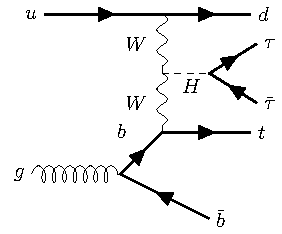
\includegraphics[width=0.45\textwidth]{/cephfs/user/s6chkirf/feynman_diagrams/tHq_tautau}\\
      \includegraphics[width=0.45\textwidth]{/cephfs/user/s6chkirf/feynman_diagrams/tHq_WW}
      \includegraphics[width=0.45\textwidth]{/cephfs/user/s6chkirf/feynman_diagrams/tHq_ZZ}
      \begin{itemize}
        \item n-jets: 2 (b-jets: \textbf{1})
        \item b-jet WP: 70 DL1r
        \item nLeptons \& nTaus: \bf{$1e / \mu~2\tau_{\text{had}}$}
        \item $E_{\text{T,miss}}$: no cut (to \SI{800}{GeV})
      \end{itemize}
    \end{column}
    \begin{column}{0.7\textwidth}
      \vspace*{-0.05\textwidth}
      \begin{itemize}
        \footnotesize
        \item jets:
        \vspace*{-0.02\textwidth}
        \begin{itemize}
          \footnotesize
          \item $p_T>\SI{35}{GeV}$
          \item $|\eta|<4.5$
          \item EMPFlow
        \end{itemize}
        \item electrons:
        \vspace*{-0.02\textwidth}
        \begin{itemize}
          \footnotesize
          \item $p_T>\SI{20}{GeV}$ leading \SI{27}{GeV}
          \item $|\eta|<2.5$ not in 1.37 - 1.52
          \item WP: LooseAndBLayerLH ; \\isolation: no requirement
        \end{itemize}
        \item muons:
        \vspace*{-0.02\textwidth}
        \begin{itemize}
          \footnotesize
          \item $p_T>\SI{20}{GeV}$ leading \SI{27}{GeV}
          \item $0.01<|\eta|<2.5$
          \item WP: Loose ; isolation: no requirement
        \end{itemize}
        \item taus:
        \vspace*{-0.02\textwidth}
        \begin{itemize}
          \footnotesize
          \item $p_T>\SI{20}{GeV}$ leading \SI{27}{GeV}
          \item $|\eta|<2.5$ not in 1.37 - 1.52
          \item WP: RNNLoose
          \item ASG recommended OLR ($\tau_{had}$ remove jets)
        \end{itemize}
      \end{itemize}
    \end{column}
  \end{columns}
\end{frame}
  

\begin{frame}{Challenges}
    \begin{block}{Handling of negative weights}
        \begin{itemize}
            \item What is the origin of negative3 weights
            \item How do they affect neural networks
            \item How should they be handled
        \end{itemize}
    \end{block}
    \begin{block}{Weighting of background processes}
        \begin{itemize}
            \item Dominating background can diminish the significance of secondary backgrounds in Training
            \item Adjust the network to handle several levels of background.
        \end{itemize}
    \end{block}
    \begin{block}{Accelerating network optimisation}
        \begin{itemize}
            \item Exploration of new features is only possible in an optimised network
            \item To minimise the work of constant optimisation
        \end{itemize}
    \end{block}
\end{frame}
\begin{frame}{Background processes in neural network training}
    \begin{columns}
        \begin{column}{0.5\textwidth}
            \begin{figure}
                \centering
                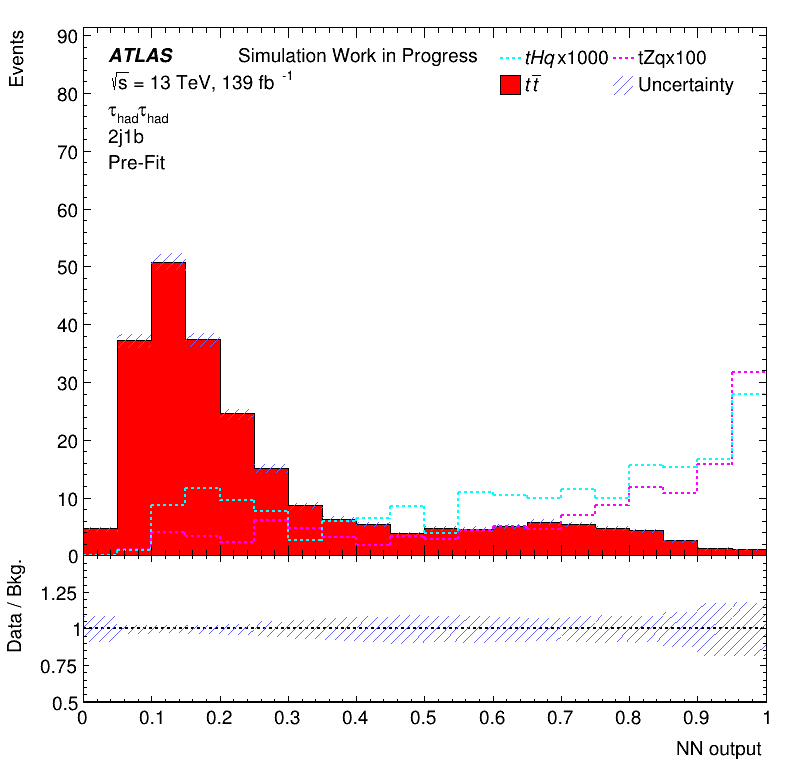
\includegraphics[width=\textwidth]{sgBkgComp}
            \end{figure}
        \end{column}
        \begin{column}{0.5\textwidth}
            \begin{itemize}
                \item \ttbar dominates the training
                \vspace{0.5cm}
                \item \tZq classified as signal
                \vspace{0.5cm}
                \item Approaches:
                    \begin{itemize}
                        \item multiple networks
                        \item multiple targets
                        \item reweighting samples
                    \end{itemize} 
            \end{itemize}
        \end{column}
    \end{columns}
\end{frame}
%\begin{frame}{Info about negative weights}
%    \begin{itemize}
%        \item Researching
%    \end{itemize}
%\end{frame}

\begin{frame}{Impact of negative weights on the training}
    \begin{columns}
        \begin{column}{0.5\textwidth}
            \begin{figure}
                \centering
                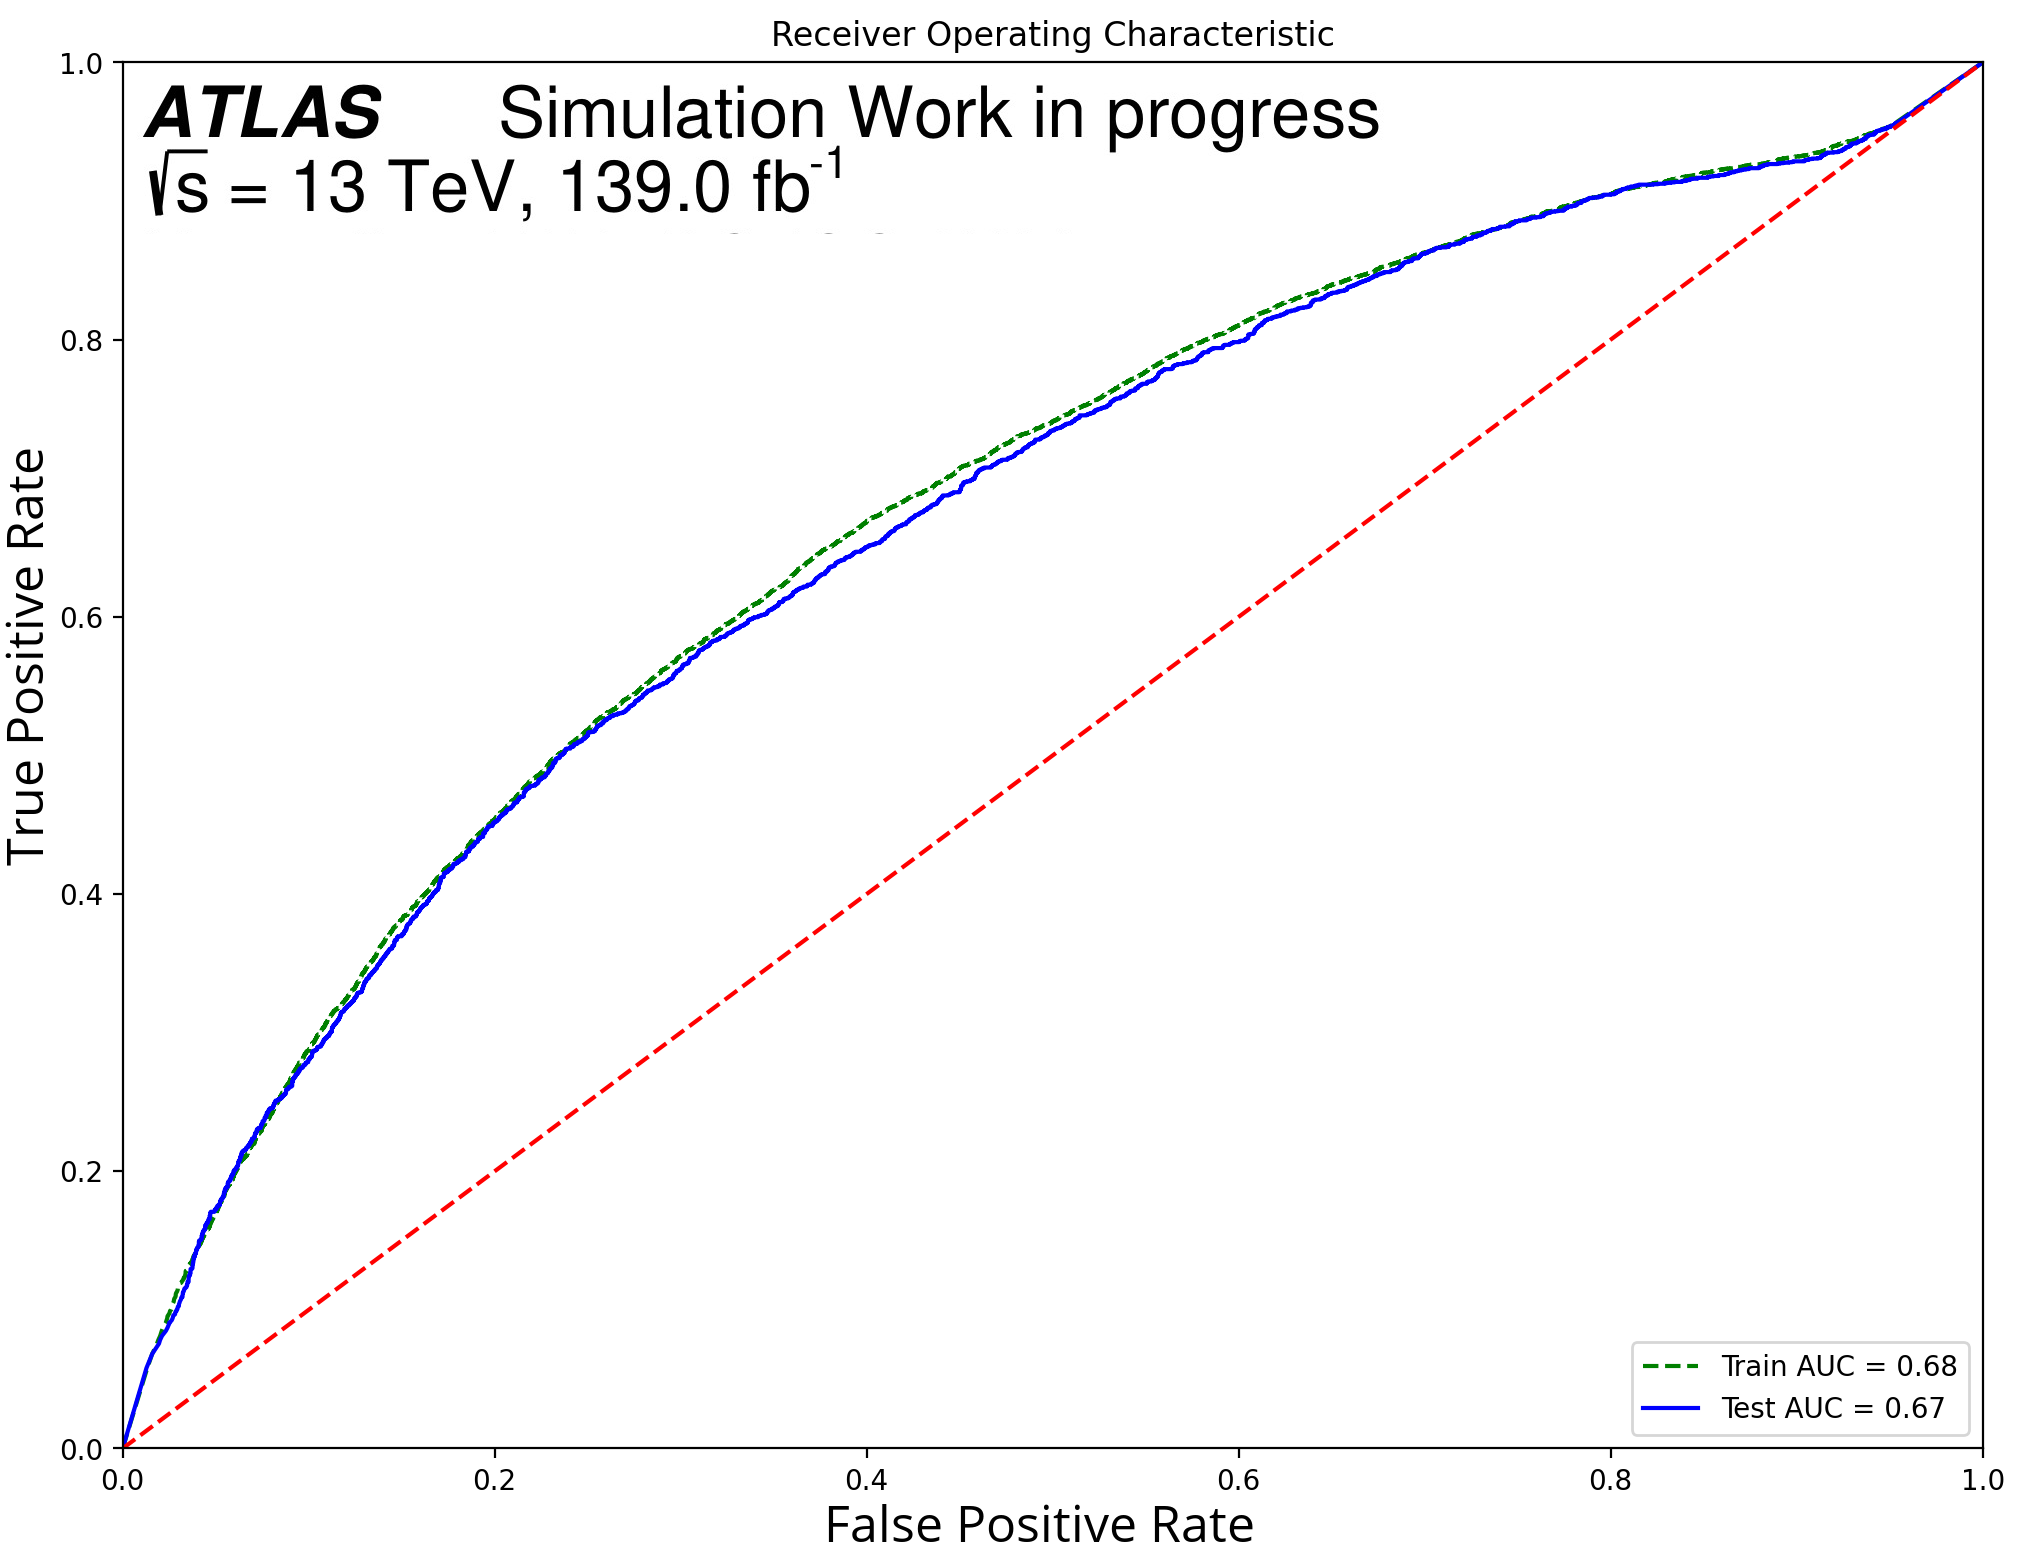
\includegraphics[width=\textwidth]{ROC_normalWeights}
            \end{figure}
        \end{column}
        \begin{column}{0.5\textwidth}
            \begin{figure}
                \centering
                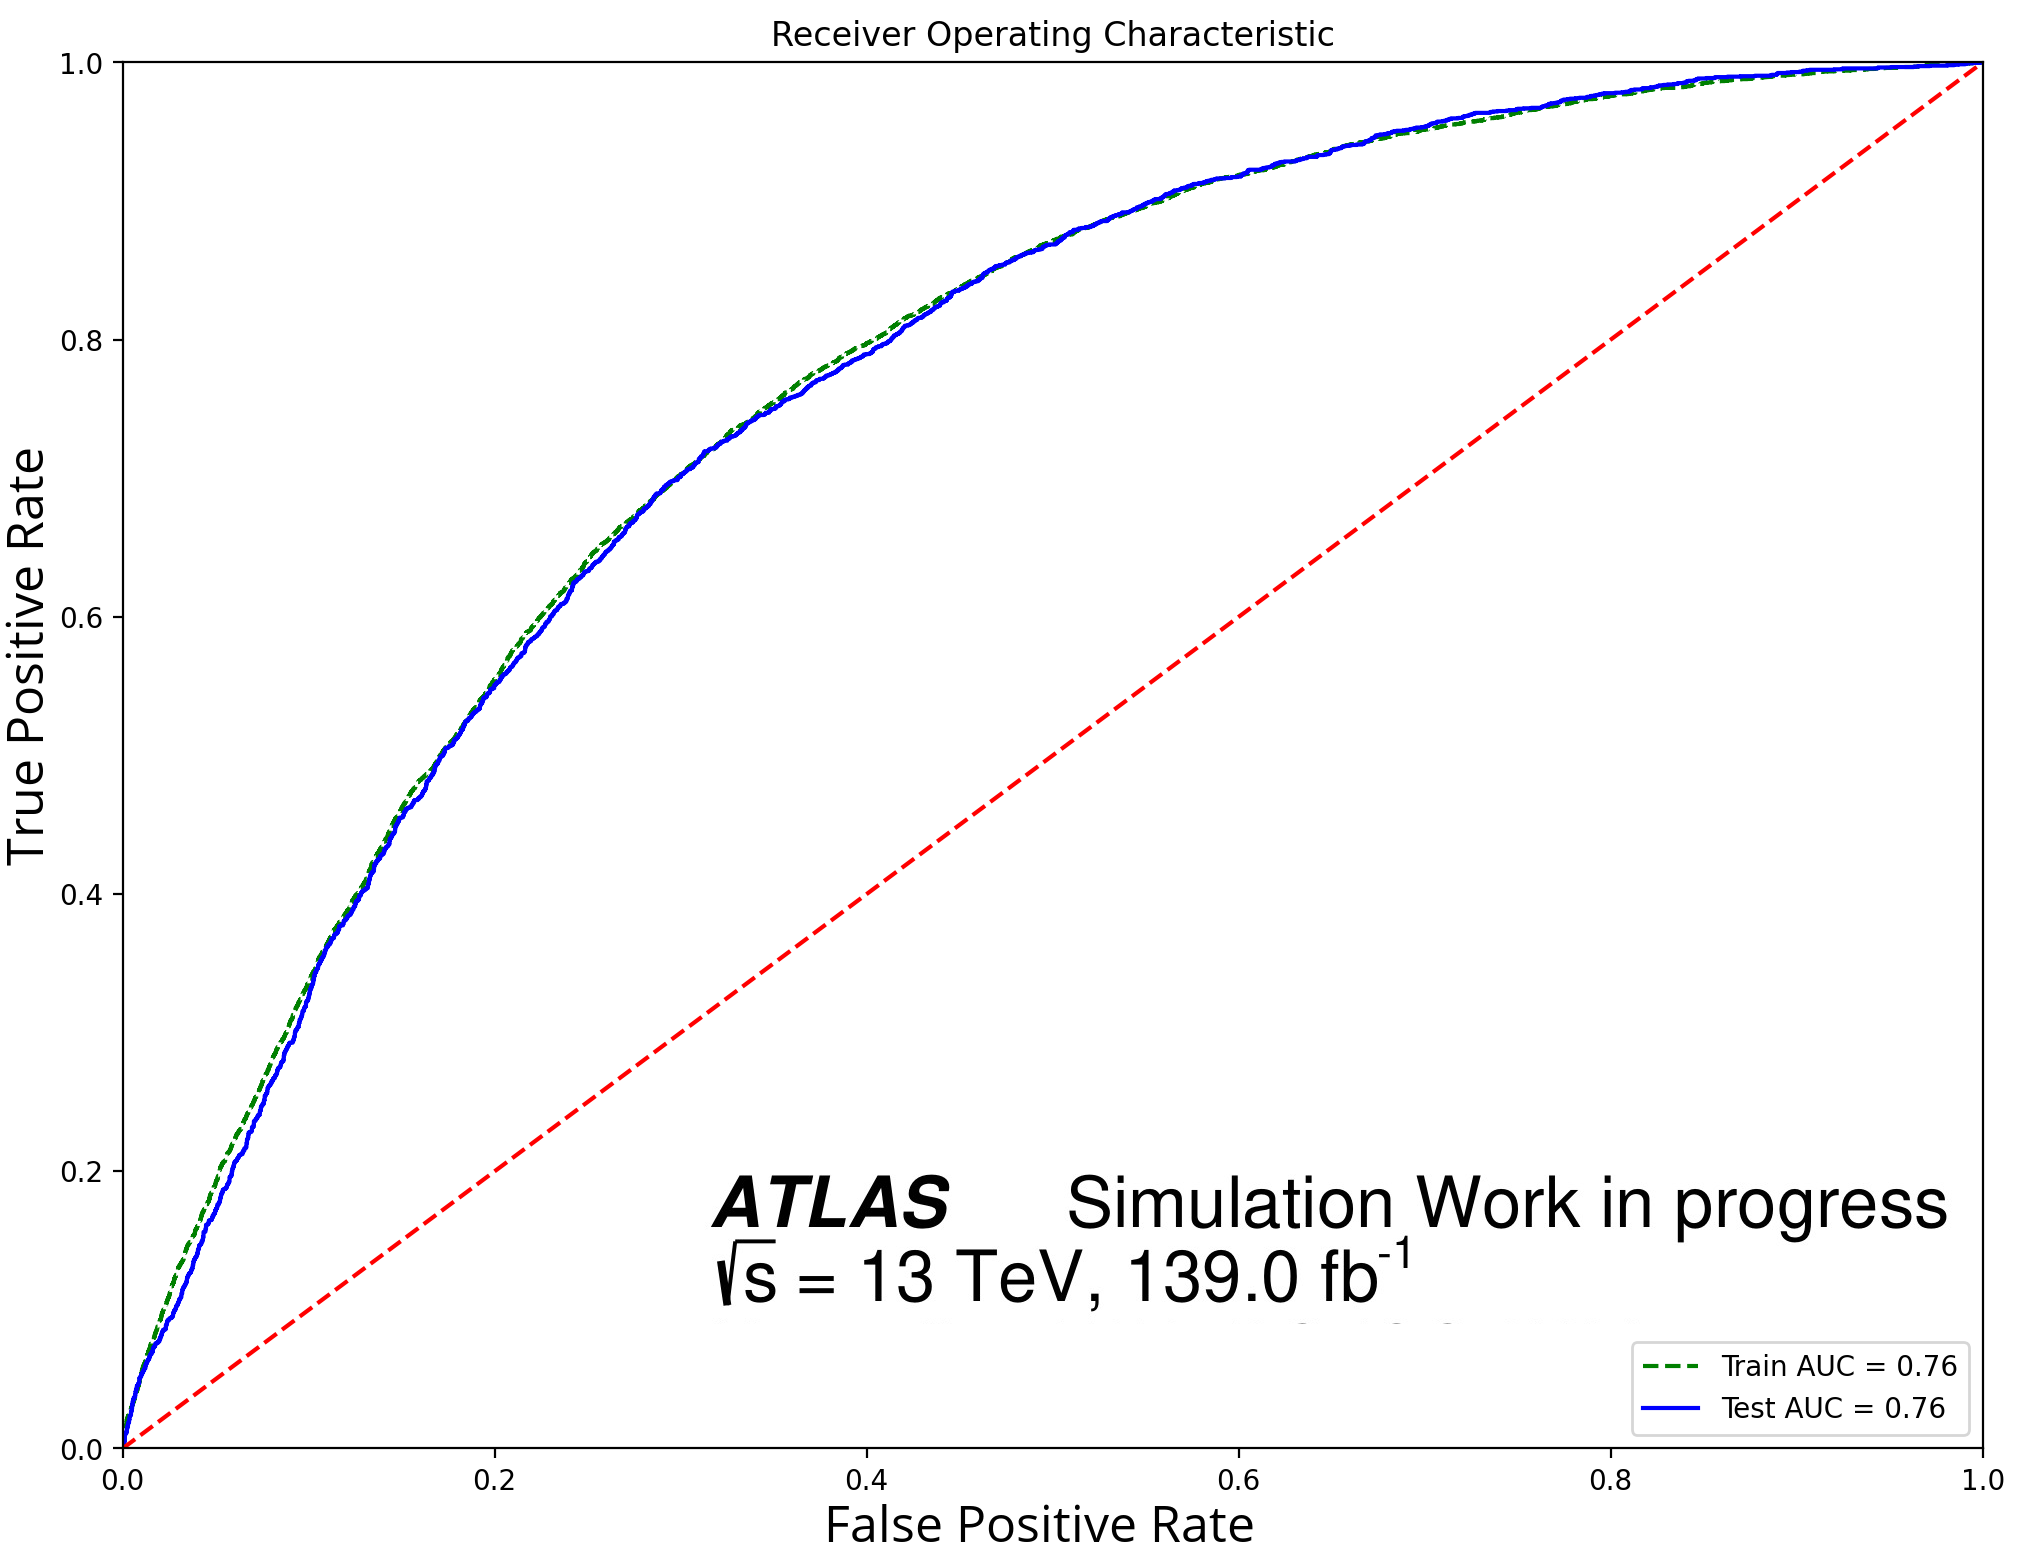
\includegraphics[width=\textwidth]{ROC_absoluteWeights}
            \end{figure}
        \end{column}
    \end{columns}
    \begin{itemize}
        \item About $35 \%$ of events have negative weights
        \item Negative weights break the networks training
        \item Possible ways of handling the weights is to use the absolutes or just use positive weights
    \end{itemize}
\end{frame}
\begin{frame}{Problems in network optimisation}
    \begin{block}{Obstacles of optimisation processes}
        \begin{itemize}
            \item Grid searches are both tedious and resource intensive
            \item Knowledge gained in one problem is rarely universal
            \item Experienced users can develop a bias towards certain hyperparamters
        \end{itemize}
    \end{block}
    \begin{block}{Applications of evolutionary optimisation}
        \begin{itemize}
            \item A neural network should be developed in parallel to an ongoing analysis.
            \item New additions need a new optimisation.
        \end{itemize}
    \end{block}
\end{frame}

%\begin{frame}{Training specifications (Redundant?) }
%  \begin{itemize}
%      \item Training a deep neural network
%      \vspace{0.2cm}
%      \item Coarse optimisation using an evolutionary neural network
%      \vspace{0.2cm}
%      \item Fine optimisation doing a grid search
%      \vspace{0.2cm}
%      \item Optimised hyperparameters:
%          \begin{itemize}
%              \item Number of nodes
%              \item Number of layers
%              \item Dropout percentage
%          \end{itemize}
%      \item Signal: \tHq
%      \item Background: \ttbar
%      \item Using absolute weights
%  \end{itemize}
%\end{frame}

\begin{frame}{Evolutionary optimisation of neural networks}
    \begin{itemize}
        \item Combination of a grid searches with a survival of the fittest setup
        \vspace{0.2cm}
        \item Start with a number of random hyperparamters
        \vspace{0.2cm}
        \item Evaluate the set of hyperparameters
        \vspace{0.2cm}
        \item Create a a new set of networks based on the previous best
        \vspace{0.2cm}
        \item Add recombination and variation to avoid local minima and bias
    \end{itemize}
\end{frame}



\begin{frame}{Example of an evolutionary training}
    \begin{columns}
        \begin{column}{0.5\textwidth}
            \vspace{-0.4cm}
            \begin{itemize}
                \item Signal: \tHq
                \vspace{0.3cm}
                \item Background: \ttbar
                \vspace{0.3cm}
                \item Testing: nodes, layers, dropout
                \vspace{0.3cm}
                \item Fixed hyperparameters:
                    \begin{itemize}
                        \item Optimizer: Adam
                        \item Activation: relu, sigmoid
                        \item Batchsize: 1000
                        \item Epochs per generation: 25
                    \end{itemize}
            \end{itemize}
        \end{column}
            \begin{column}{0.5\textwidth}
                \begin{block}{Initial parameters}
                    \begin{itemize}
                        \item Layers: $1-10$
                        \item Nodes: $1-100$
                        \item Dropout: $0-1$
                    \end{itemize}
                \end{block}
                \begin{block}{Final parameters}
                    \begin{itemize}
                        \item Layers: $4\pm2$
                        \item Nodes: $67\pm33$
                        \item Dropout: $0.4\pm0.3$
                    \end{itemize}
                \end{block}
        \end{column}
    \end{columns}
\end{frame}


%\begin{frame}{ROC and Separation}
%    \begin{columns}
%        \begin{column}{0.5\textwidth}
%            \begin{figure}
%                \centering
%                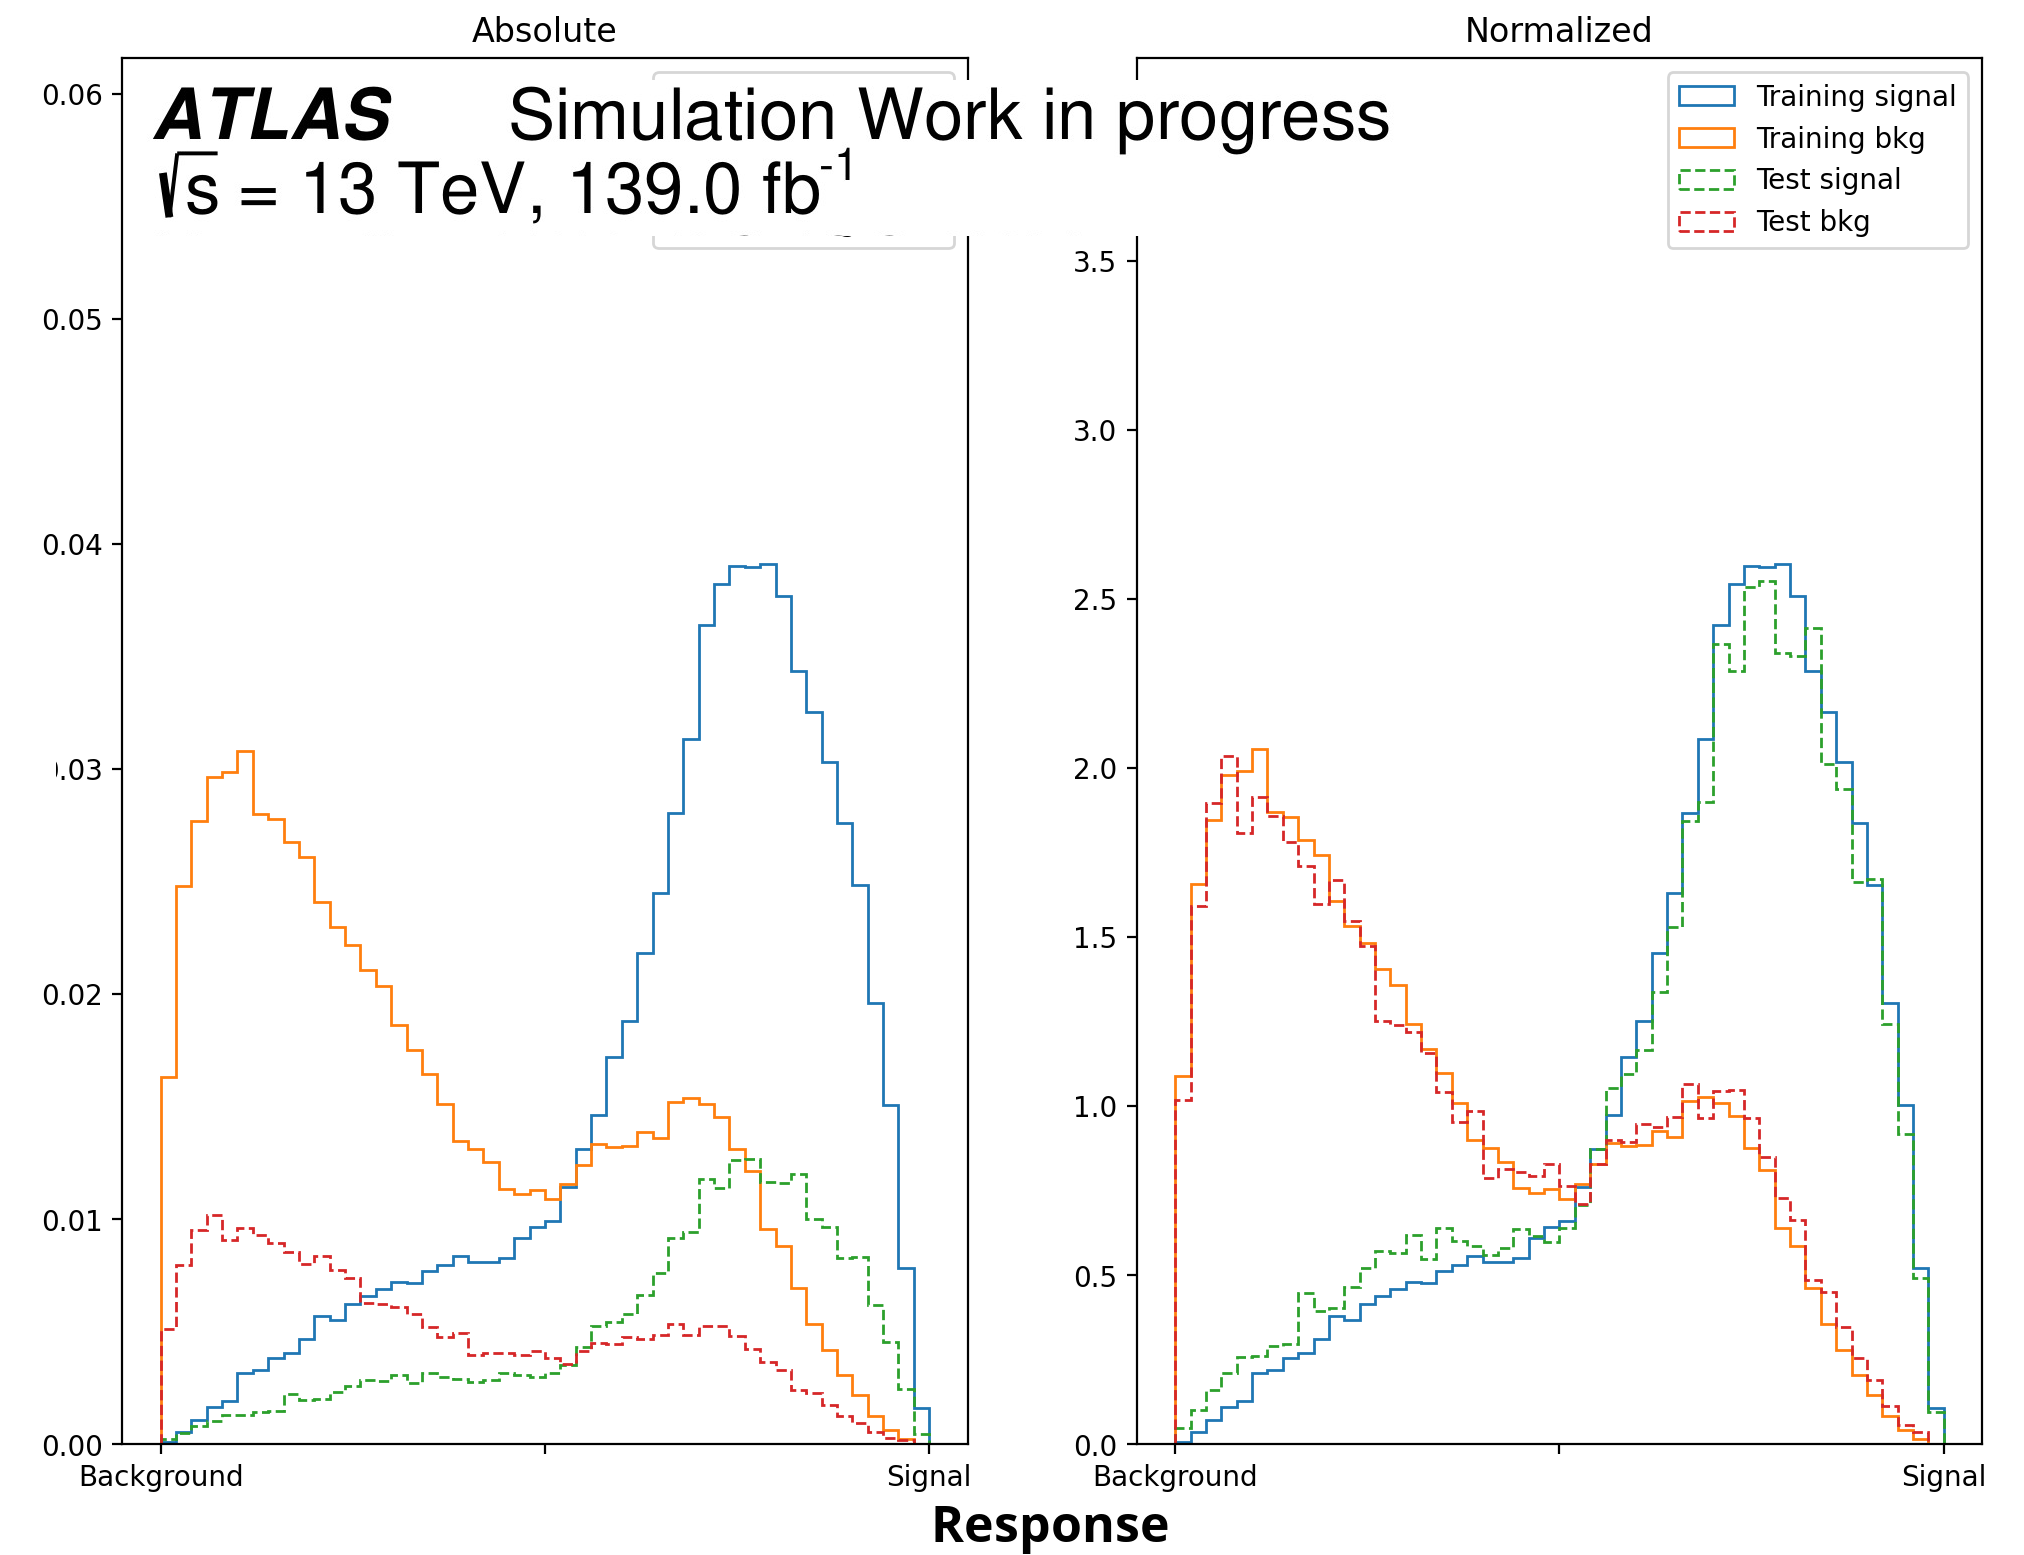
\includegraphics[width = \textwidth]{evo_response.png}
%            \end{figure}
%        \end{column}
%        \begin{column}{0.5\textwidth}
%            \begin{figure}
%                \centering
%                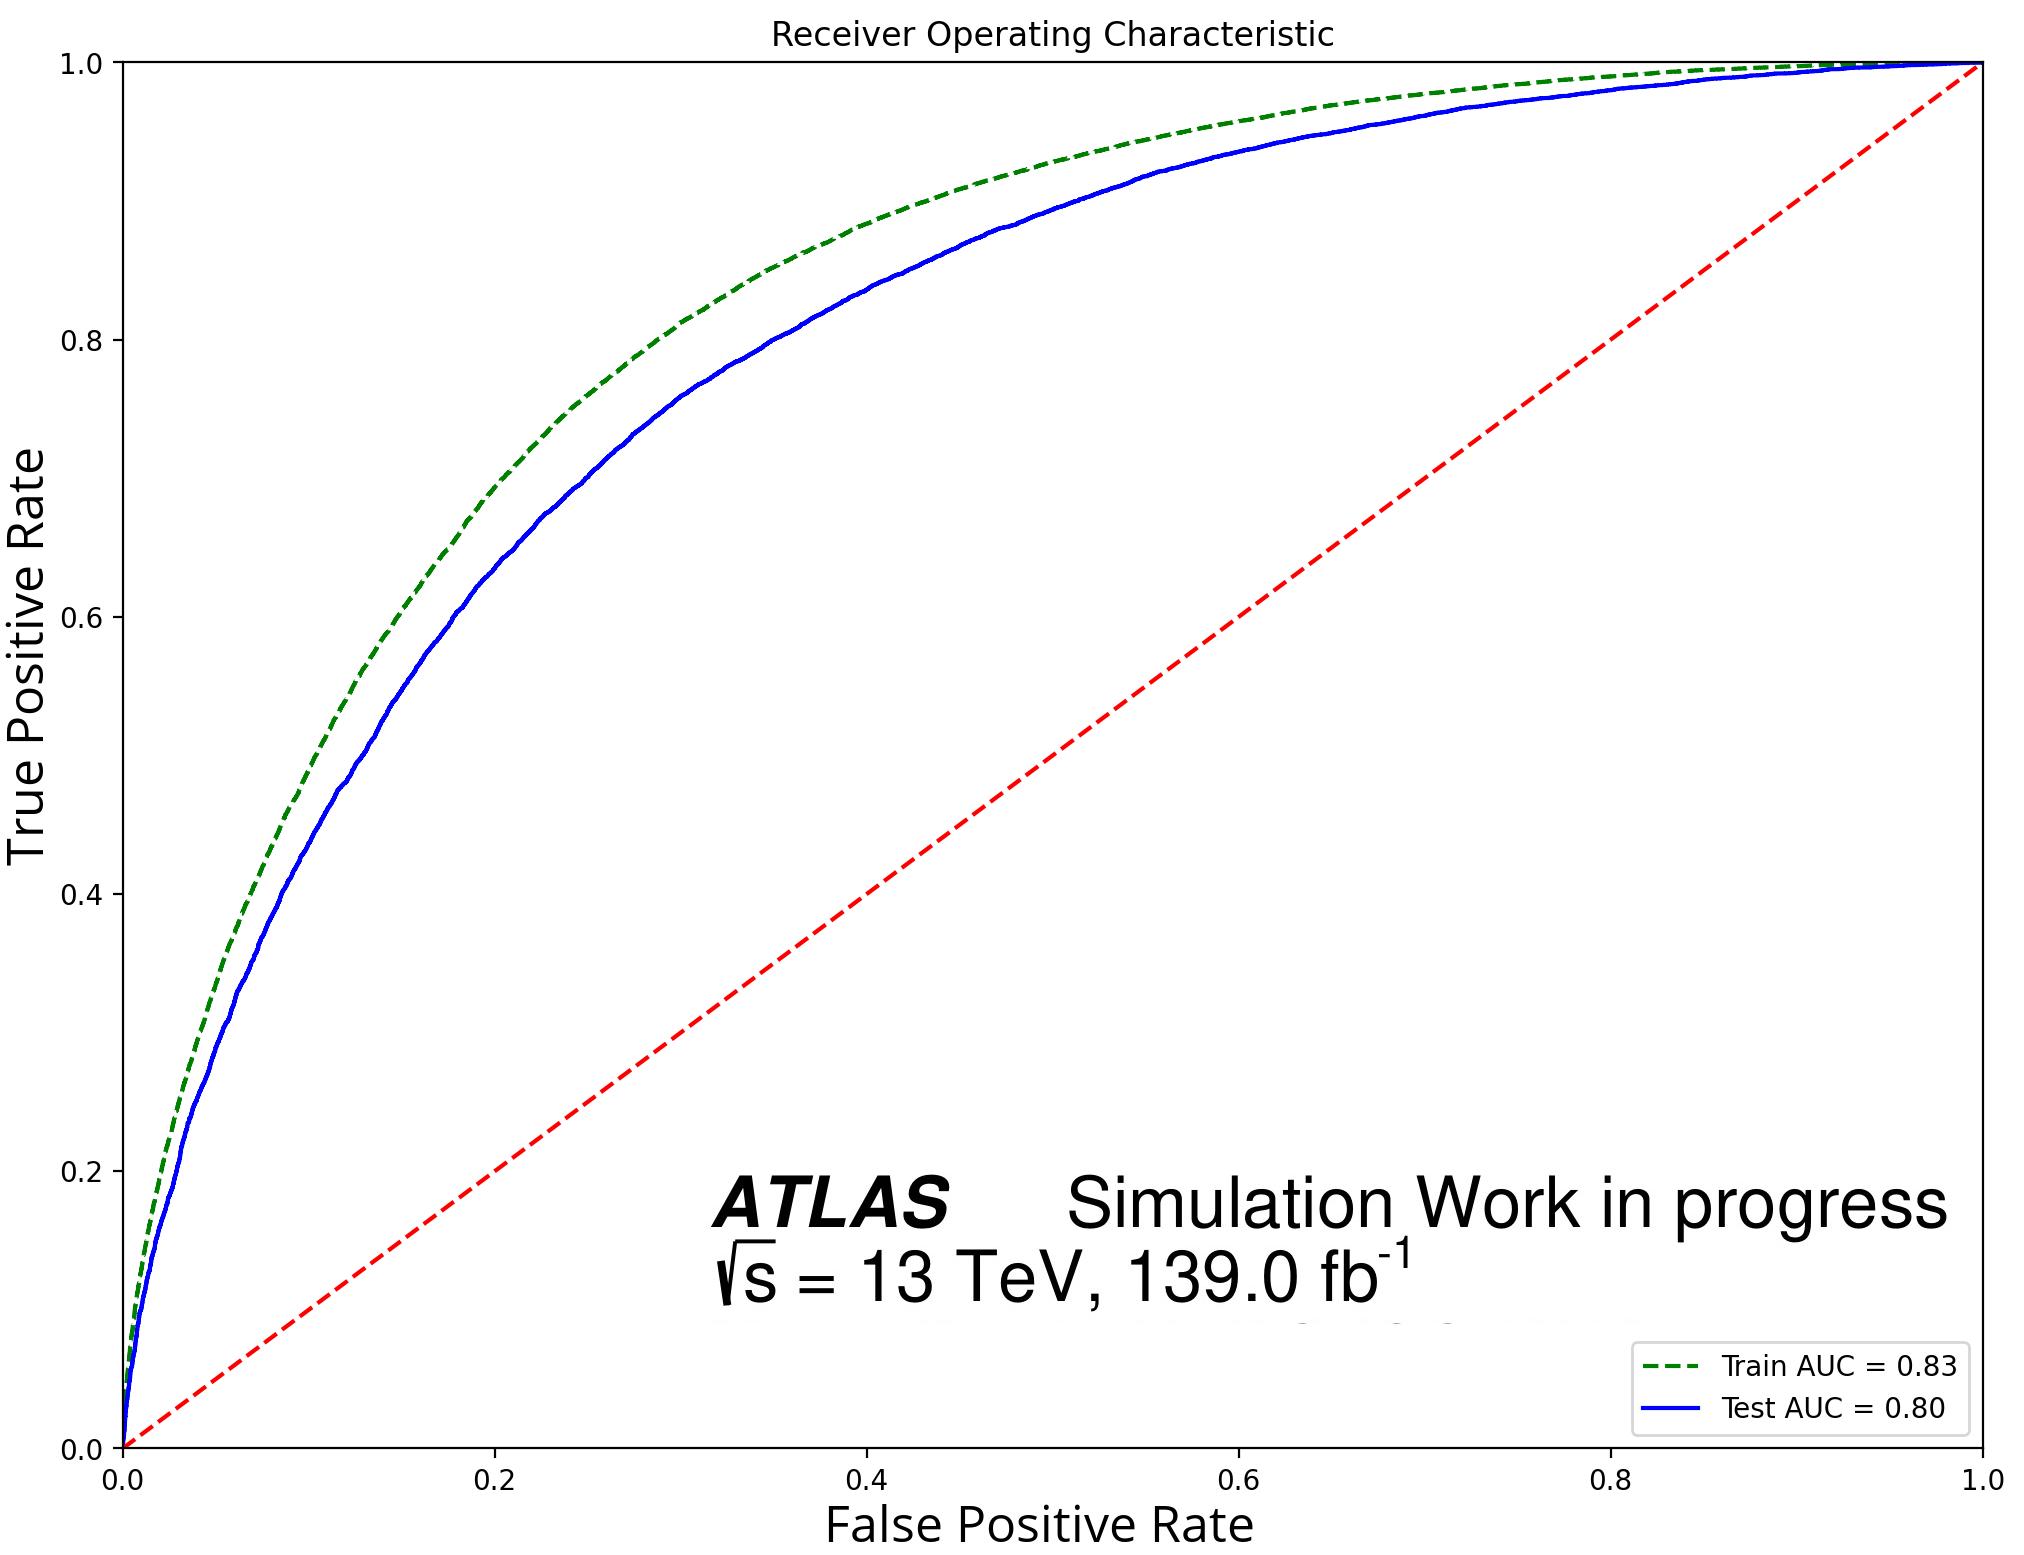
\includegraphics[width = \textwidth]{evo_ROC.png}
%            \end{figure}
%        \end{column}
%    \end{columns}
%\end{frame}

\begin{frame}{Comparing ROC to a grid search}
    \begin{columns}
        \begin{column}{0.5\textwidth}
            \begin{figure}
                \centering
                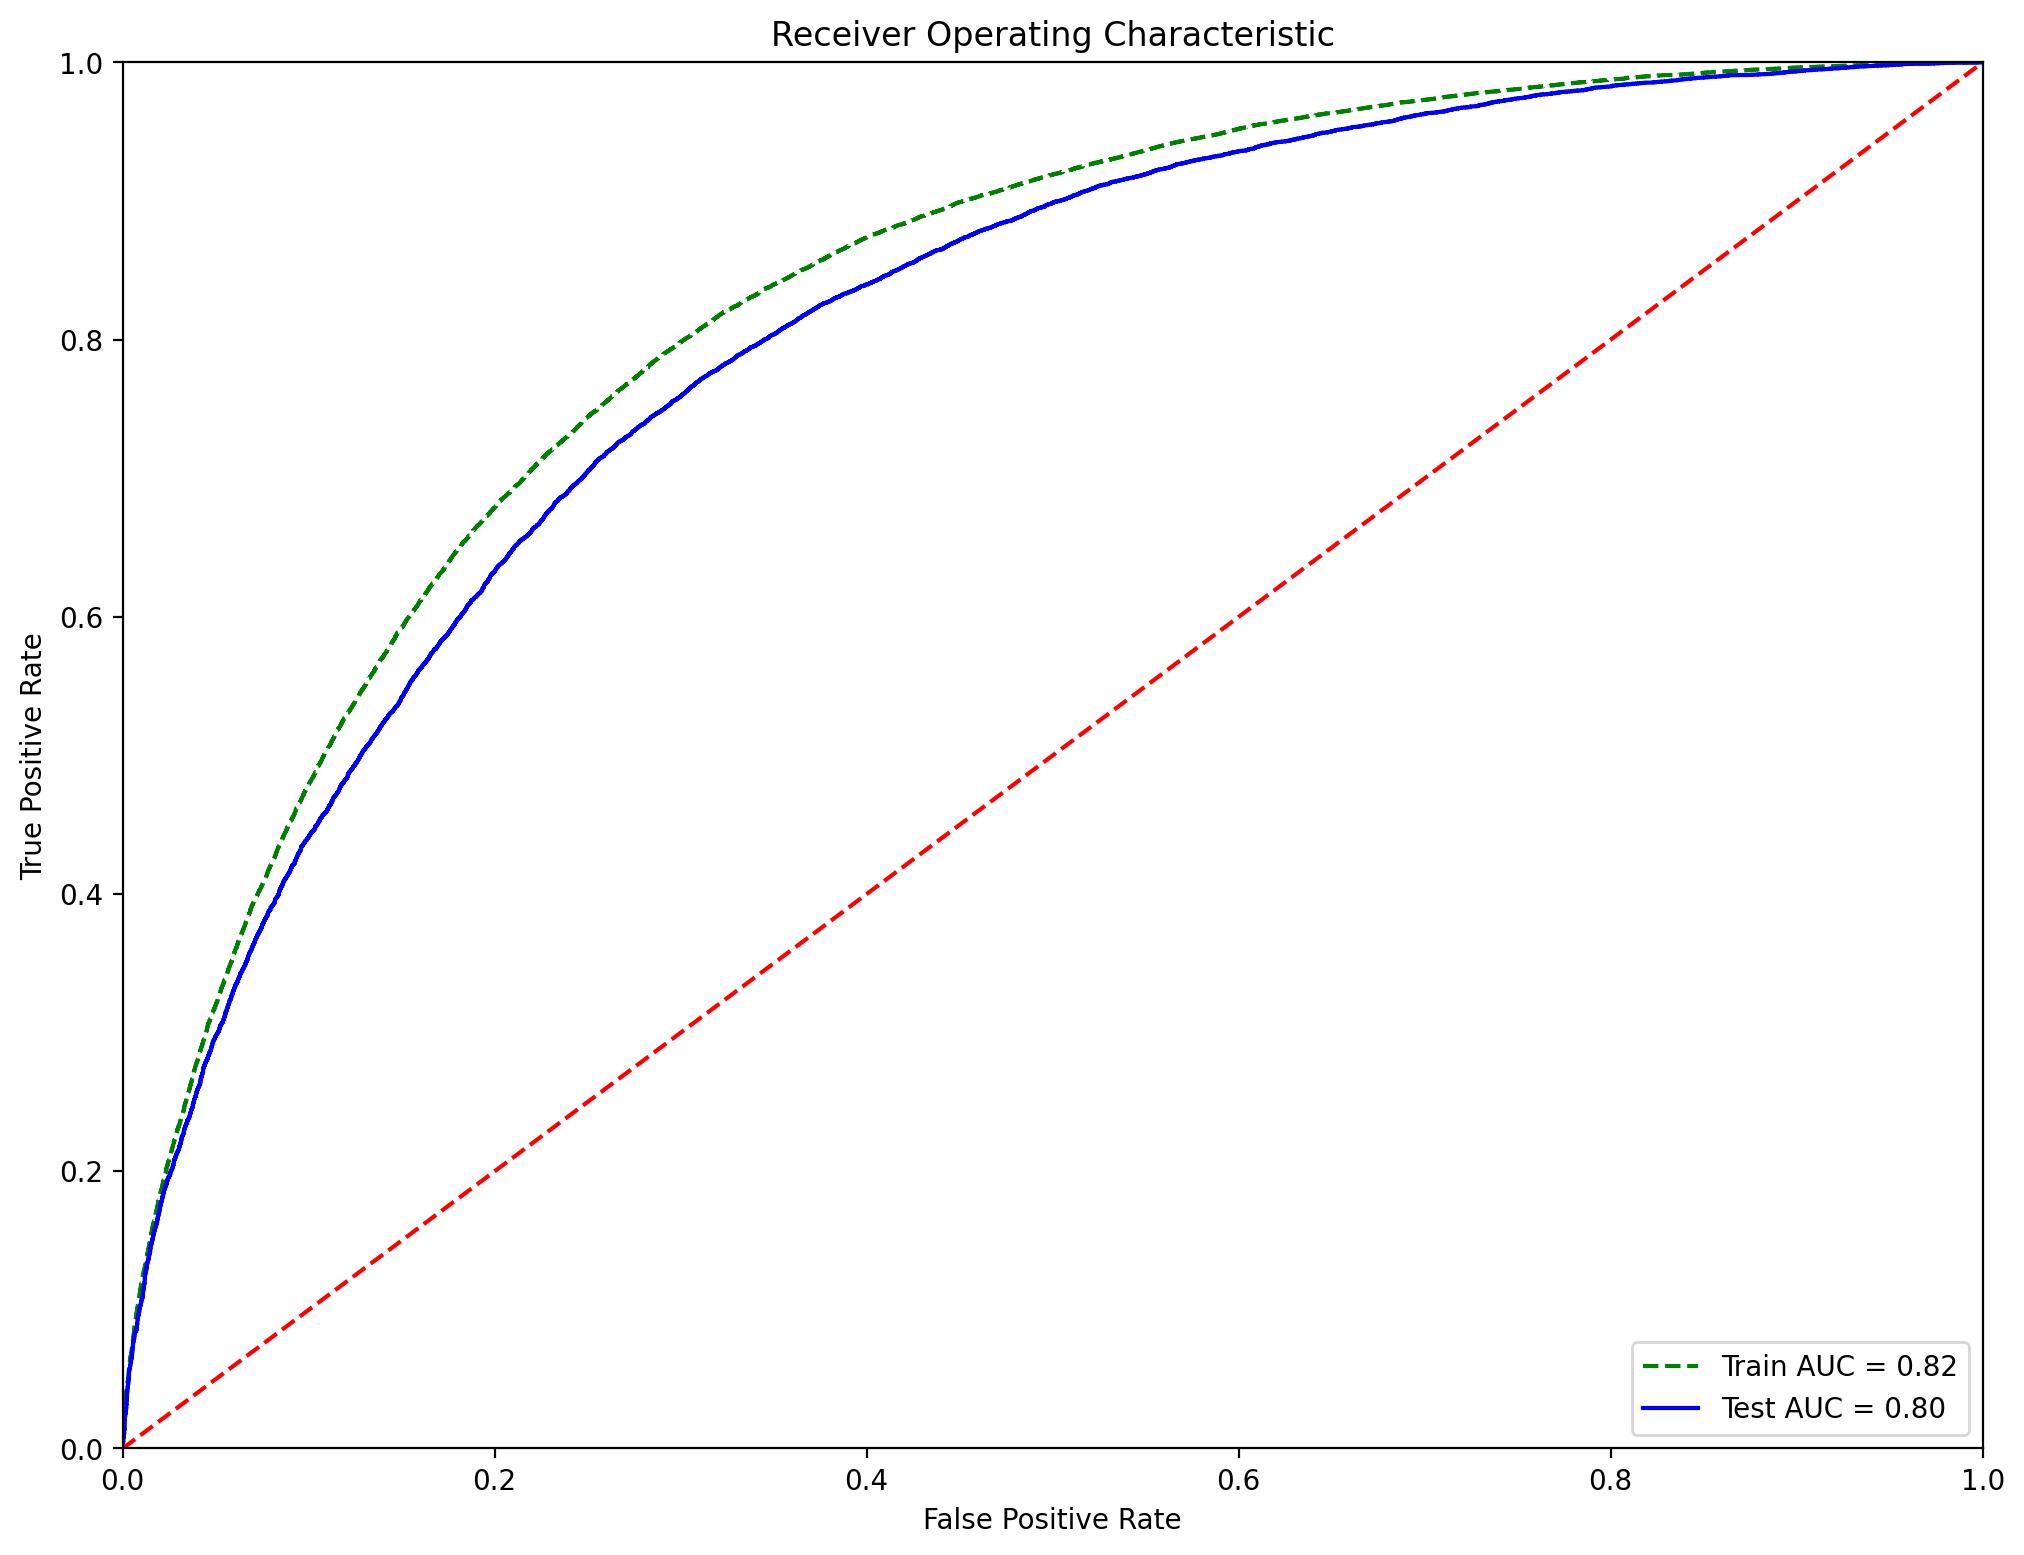
\includegraphics[width = \textwidth]{grid_ROC.png}
                \caption{Grid search}
            \end{figure}
        \end{column}
        \begin{column}{0.5\textwidth}
            \begin{figure}
                \centering
                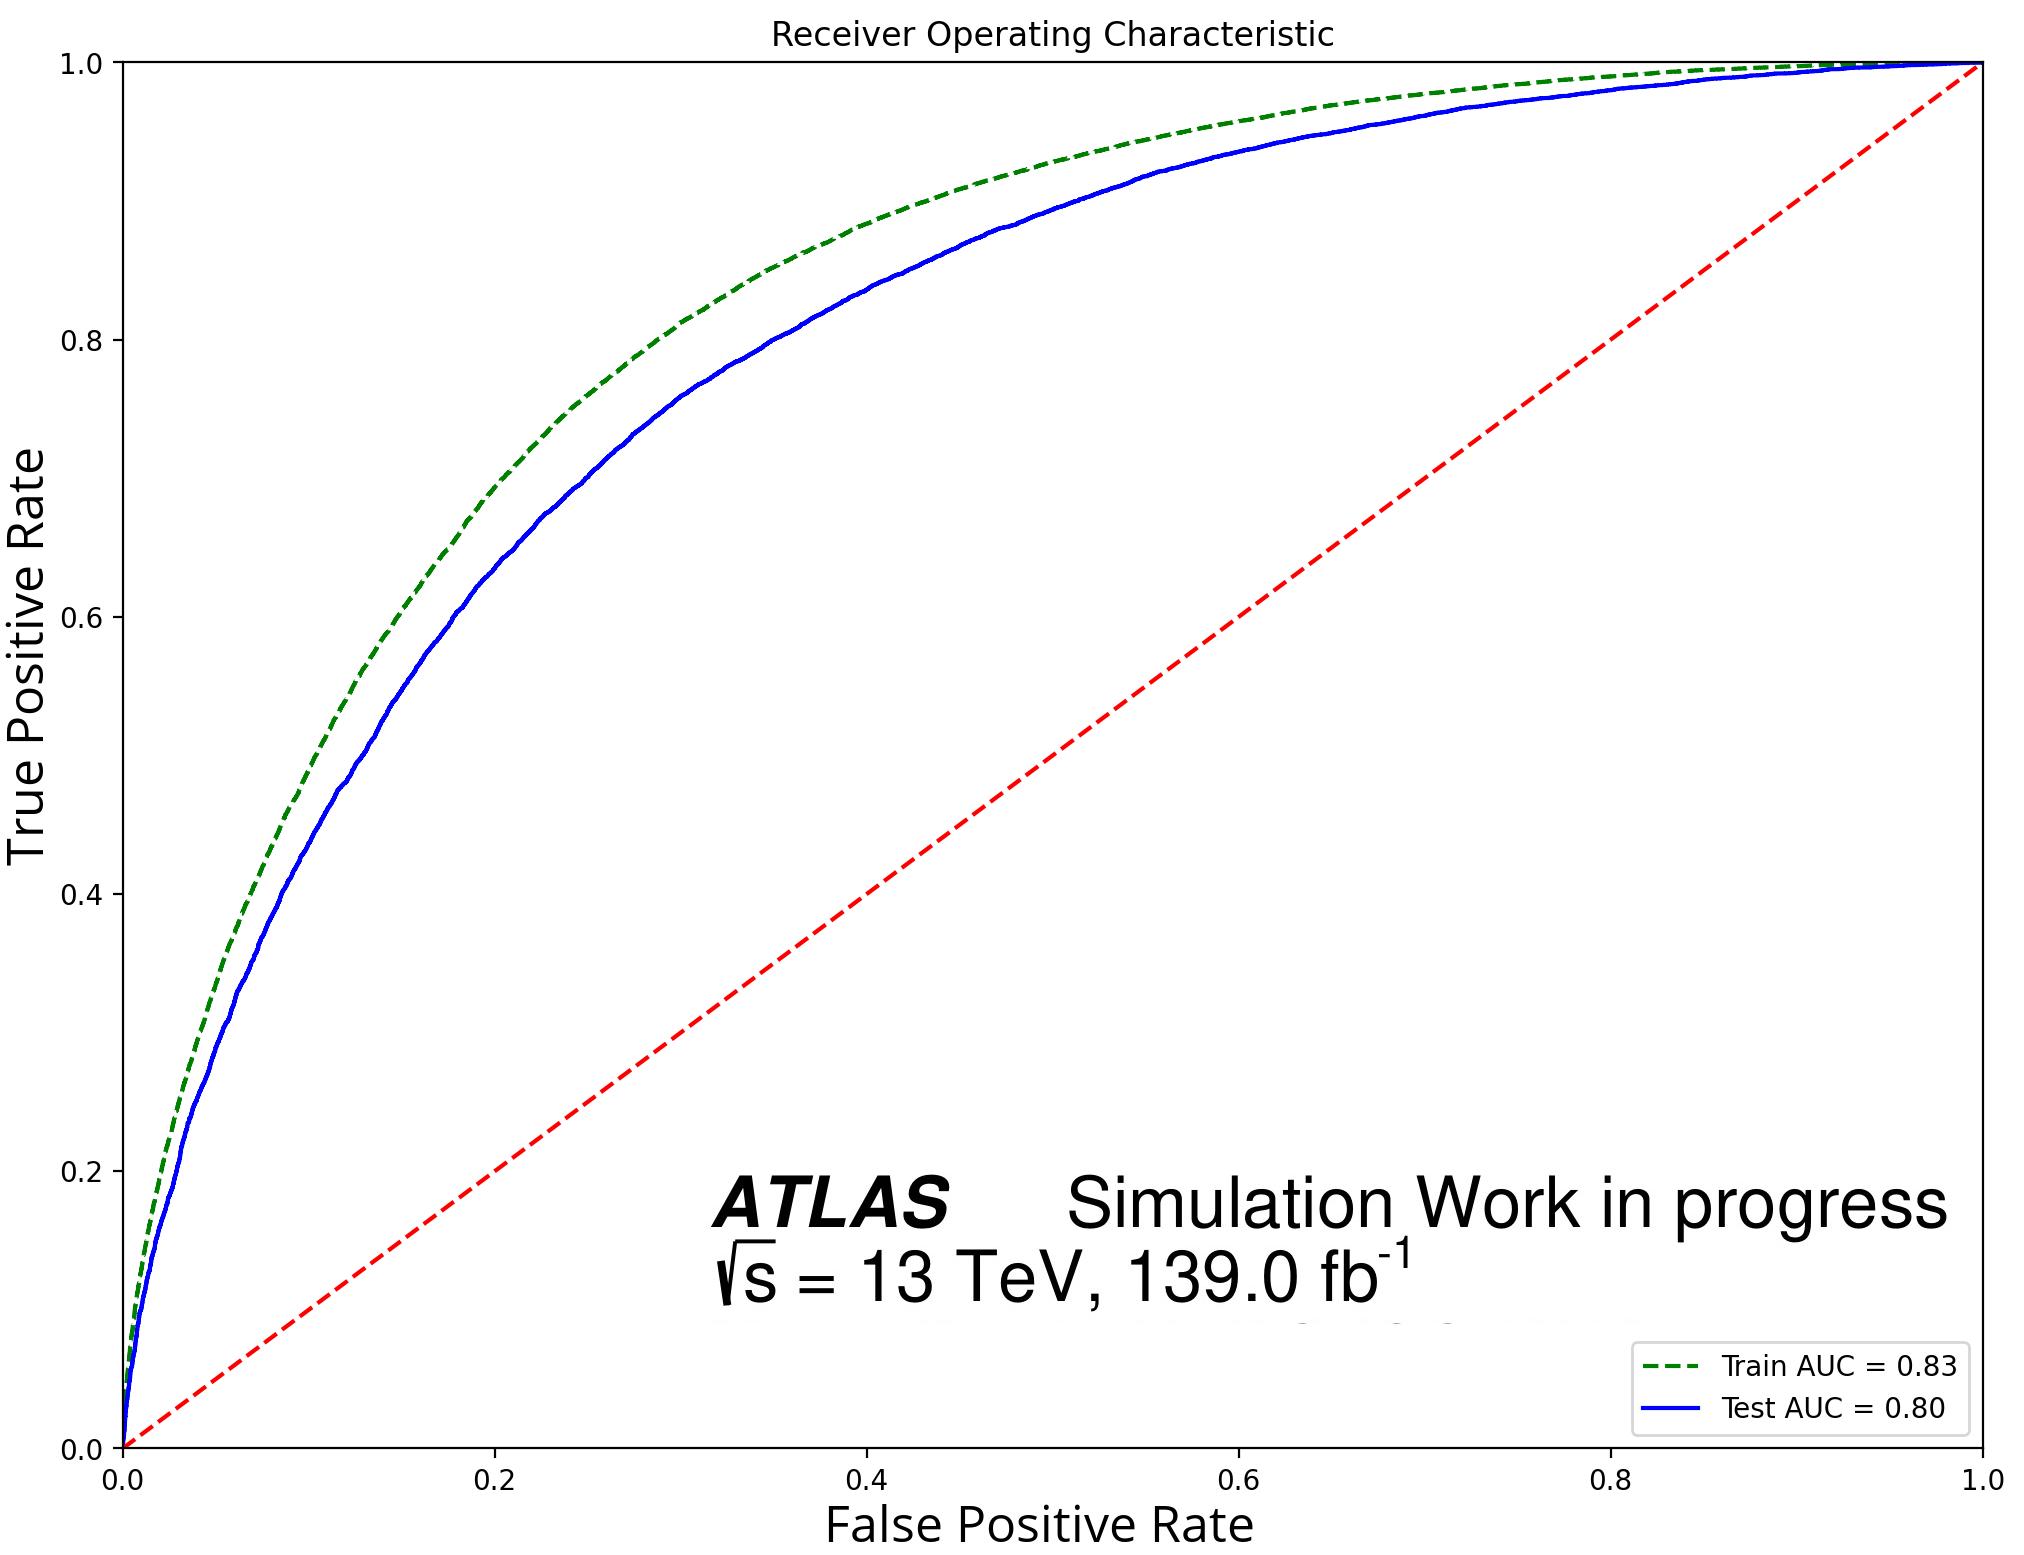
\includegraphics[width = \textwidth]{evo_ROC.png}
                \caption{Evolutionary search}
            \end{figure}
        \end{column}
    \end{columns}
\end{frame}


\begin{frame}{Comparing response to a grid search}
    \begin{columns}
        \begin{column}{0.5\textwidth}
            \begin{figure}
                \centering
                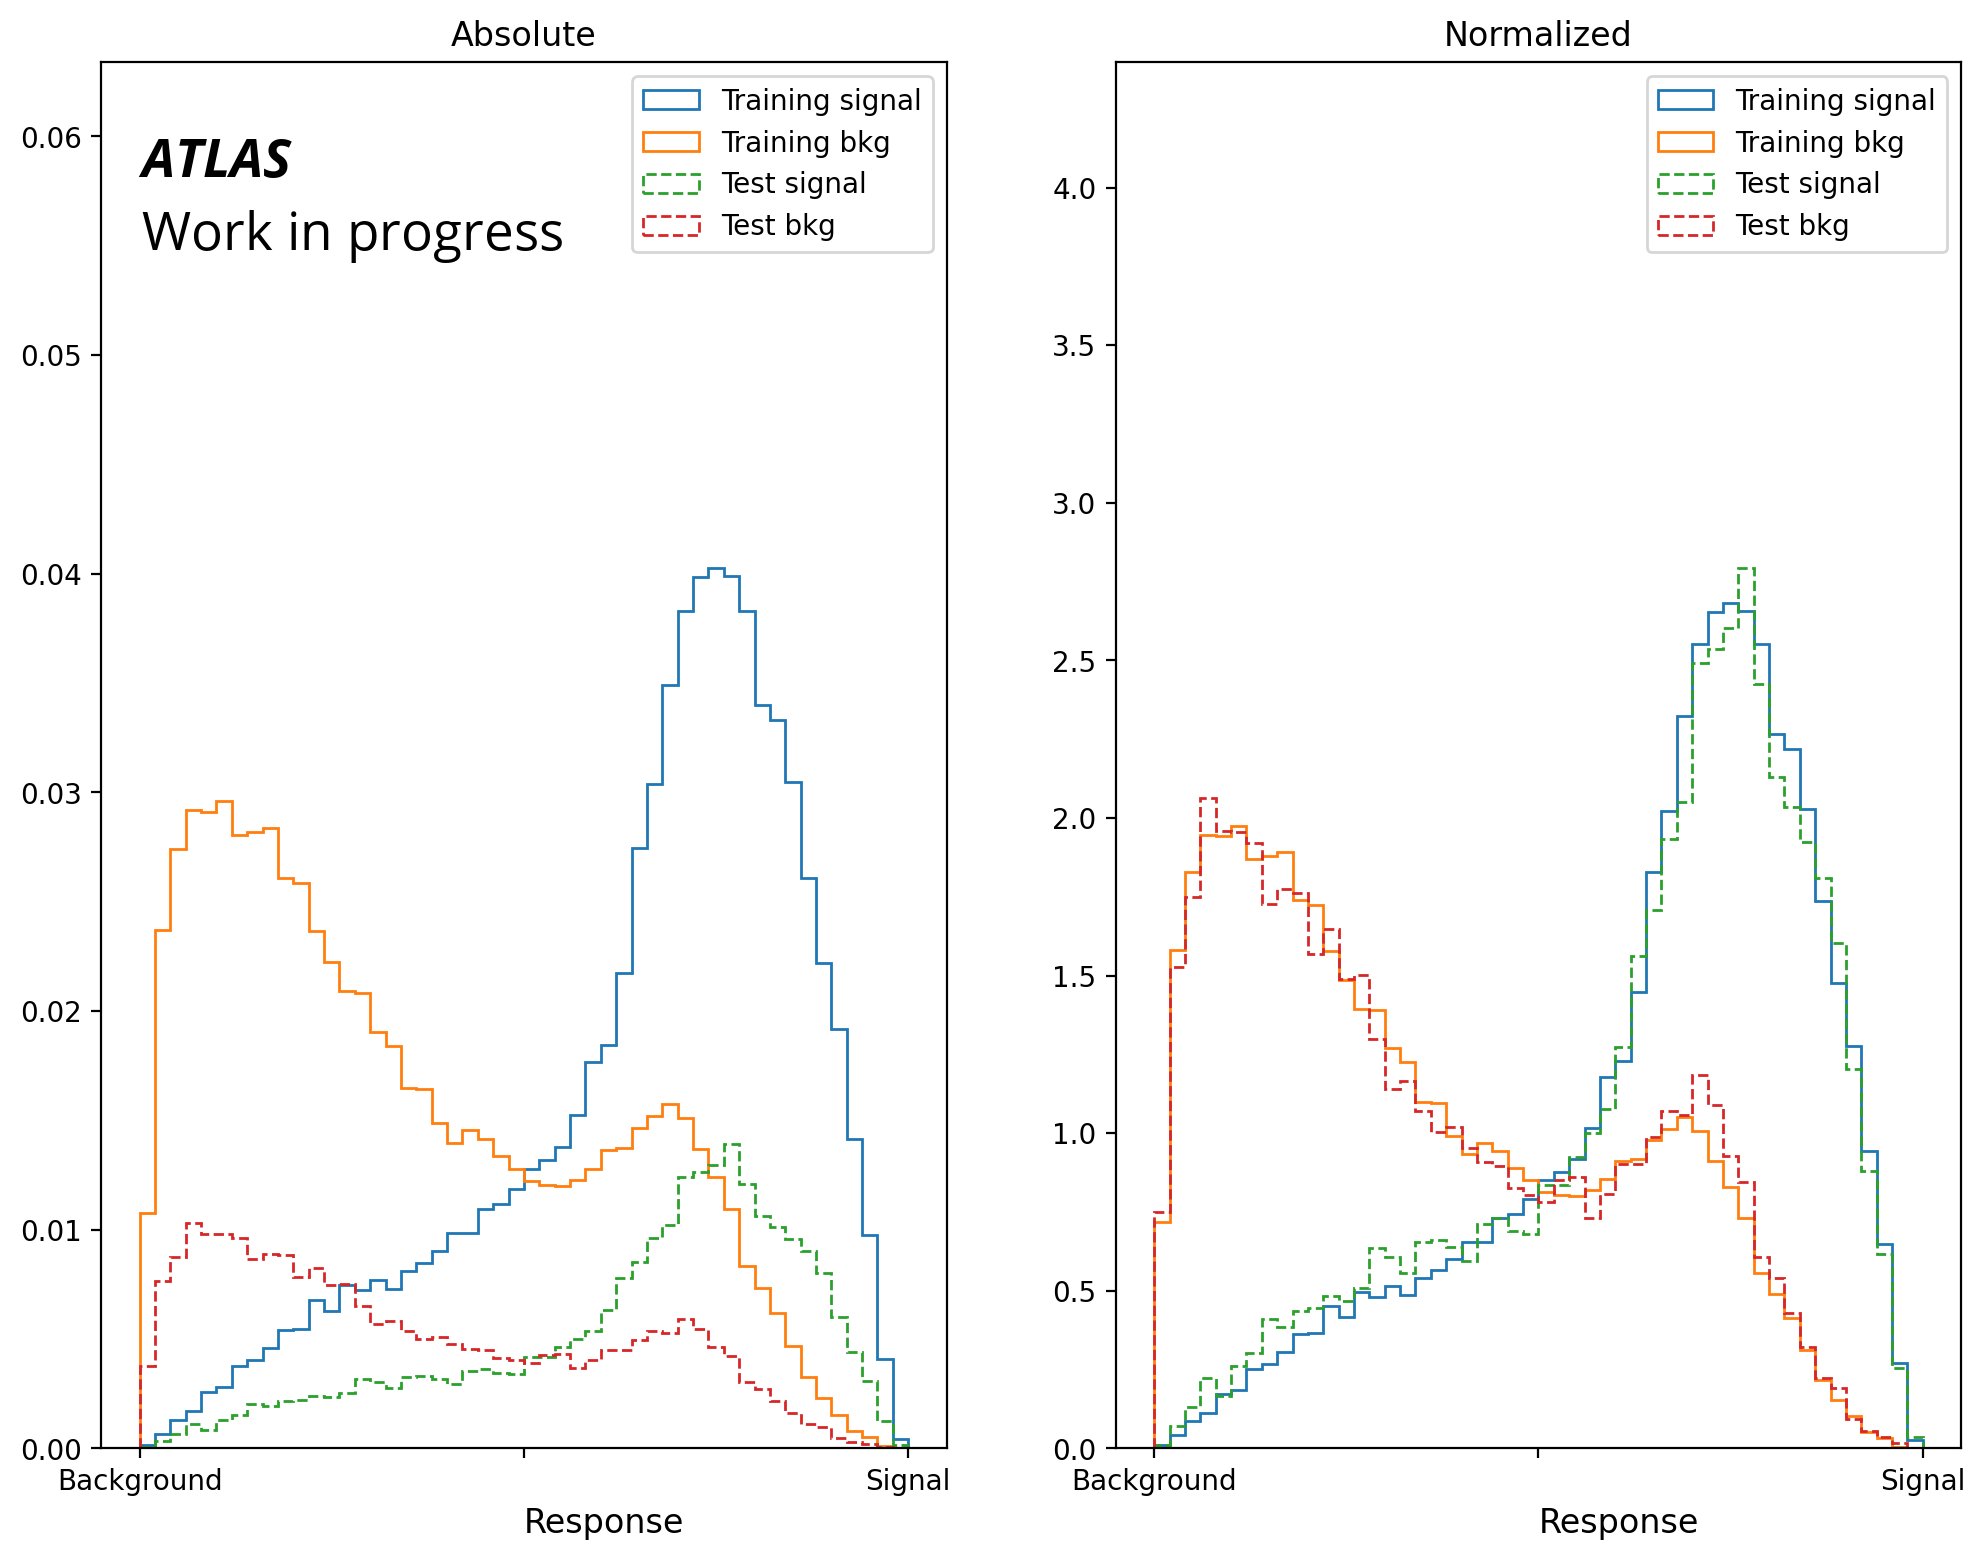
\includegraphics[width = \textwidth]{grid_response.png}
                \caption{Grid search}
            \end{figure}
        \end{column}
        \begin{column}{0.5\textwidth}
            \begin{figure}
                \centering
                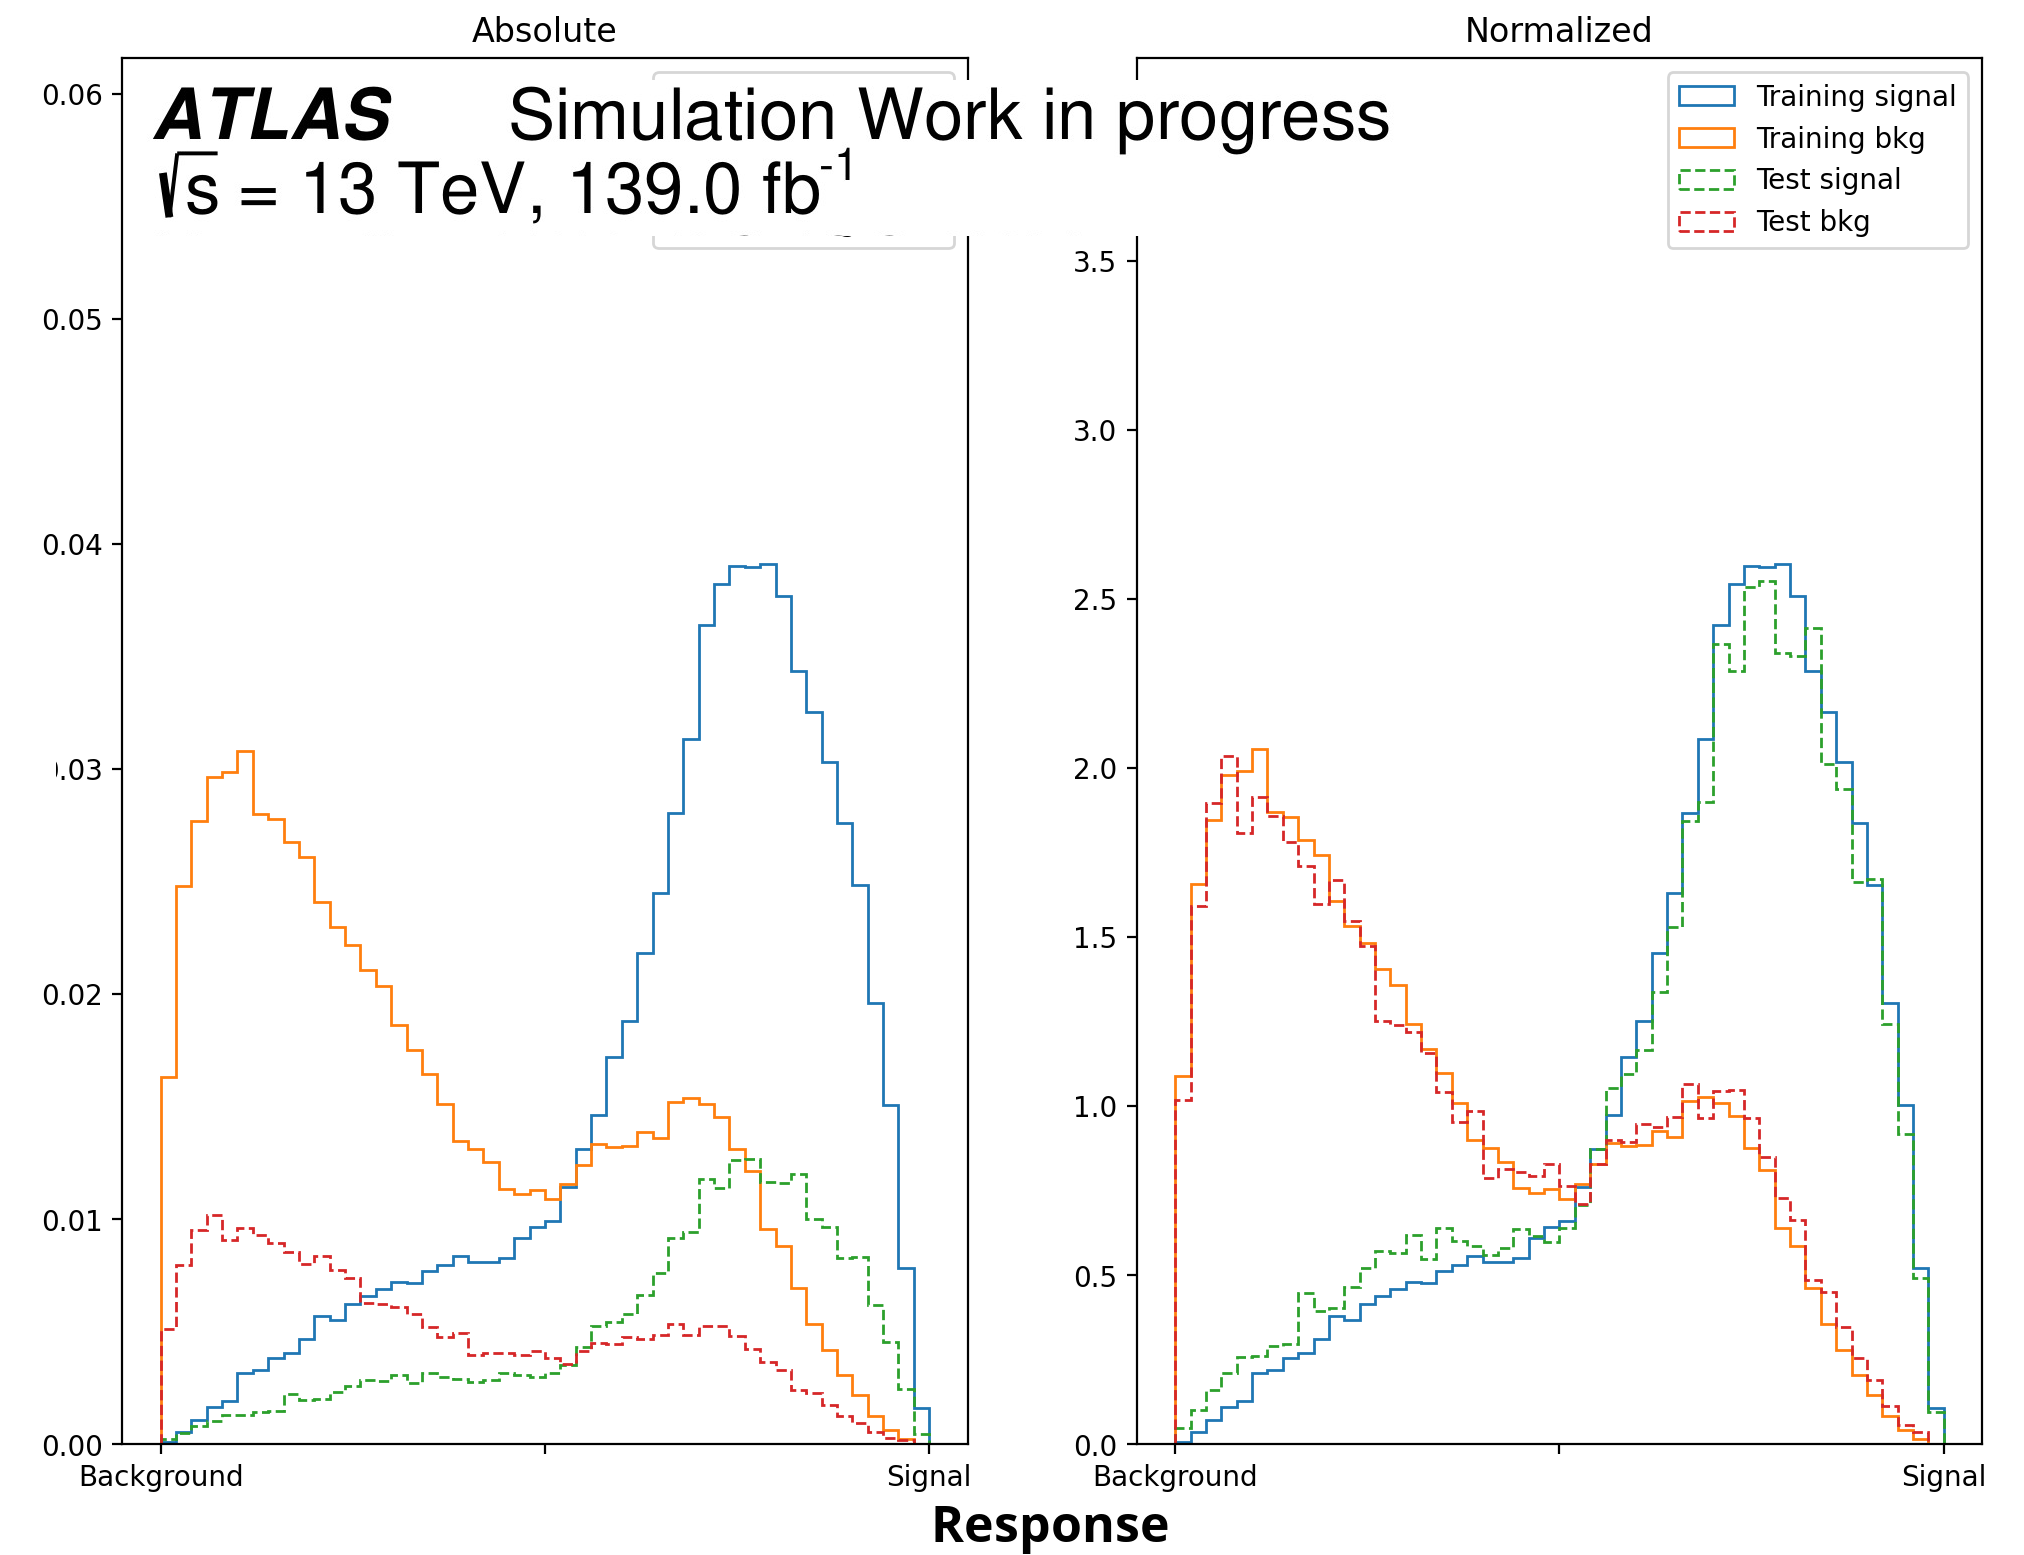
\includegraphics[width = \textwidth]{evo_response.png}
                \caption{Evolutionary search}
            \end{figure}
        \end{column}
    \end{columns}
\end{frame}
\begin{frame}{Conclusions}
    \begin{itemize}
        \item Neural networks in the \tHq channel is a \textbf{challenging} analysis.
        \vspace{0.2cm}
        \item \textbf{Negative} weights resulting from Monte Carlo generators \textbf{cannot} easily be handled by machine learning algorithms.
        \vspace{0.2cm}
        \item Different sizes of background samples result in smaller backgrounds getting \textbf{ignored} or even \textbf{misclassified} as signal.
        \vspace{0.2cm}
        \item Evolutionary optimisation of neural networks is a nice approach to \textbf{reoptimise} a network \textbf{automatically}.
    \end{itemize}
\end{frame}
%\begin{frame}{Initial problems}
    \begin{block}{Obstacles of optimisation processes}
        \begin{itemize}
            \item Grid searches are both tedious and ressource intensive
            \item Knowledge gained in one problem is rarely universal
            \item Experienced users can develop a bias towards certain hyperparamters
        \end{itemize}
    \end{block}
    \begin{block}{Making machine learning more accesible to students}
        \begin{itemize}
            \item Physics students need increasingly high programming skills
            \item Most students actively search this challenge but appreciate the rewarded of early results
            \item Desirable to create a framework that is easy to use and allows to face some challenges later on
        \end{itemize}
    \end{block}
\end{frame}

\begin{frame}{Goals}
    \begin{block}{Network optimisation}
        \begin{itemize}
            \item Create an algorithm more efficient than a grid search
            \item The algorithm should be unbiased and avoiding local minima
        \end{itemize}
    \end{block}
    \begin{block}{Accesibility}
        \begin{itemize}
            \item A new user should have easy access
            \item The challenges for a new user should be small enough to allow a feeling of achievment
        \end{itemize}
    \end{block}
    \begin{block}{BAF compatability}
        \begin{itemize}
            \item The algorithm should utilize the BAF worker node structure
            \item Ideally it should be efficient enough to create satisfying results on CPUs
        \end{itemize}
    \end{block}
\end{frame}

\begin{frame}{Evolutionary optimisation of neural networks}
    \begin{itemize}
        \item Combination of a grid searches with a survival of the fittest setup
        \vspace{0.2cm}
        \item Start with a number of random hyperparamters
        \vspace{0.2cm}
        \item Evaluate the set of hyperparameters
        \vspace{0.2cm}
        \item Create a a new set of networks based on the previous best
        \vspace{0.2cm}
        \item Add recombination and variation to avoid local minima and bias
    \end{itemize}
\end{frame}
%\section{Setup}
%How do we train a network and which difficulties are there
%\begin{frame}{Neural Networks - Processing information}
\begin{tabular}{p{5cm}|p{5cm}}
    \begin{figure}
    	
\includegraphics[scale = 0.09]{brain}
    \end{figure}
    & 
    \begin{figure}
    	
\includegraphics[scale = 1.4]{machine}
    \end{figure} \\
  \multicolumn{1}{c|}{Humam senses} & \multicolumn{1}{c}{Input variables} \\
    \begin{itemize}
        \item Extraction of relevant info
        \item Impossible for machines
    \end{itemize}
    & 
    \begin{itemize}
      \item Preprocessed by user
      \item {e.g.} kinematic variables
    \end{itemize} \\
\multicolumn{1}{c|}{Human brain} & \multicolumn{1}{c}{Net of nodes} \\
    \begin{itemize}
        \item Web of neuron cells
        \item Input from surrounding cells
        \item Single combination $\rightarrow$ action
    \end{itemize}
    & 
    \begin{itemize}
      \item Nodes = simple processors
      \item Connected by linear function
      \item Combination forms non-linear model
    \end{itemize} 
 \end{tabular}
\end{frame}


\begin{frame}{Neural network structure}
\begin{figure}
\centering
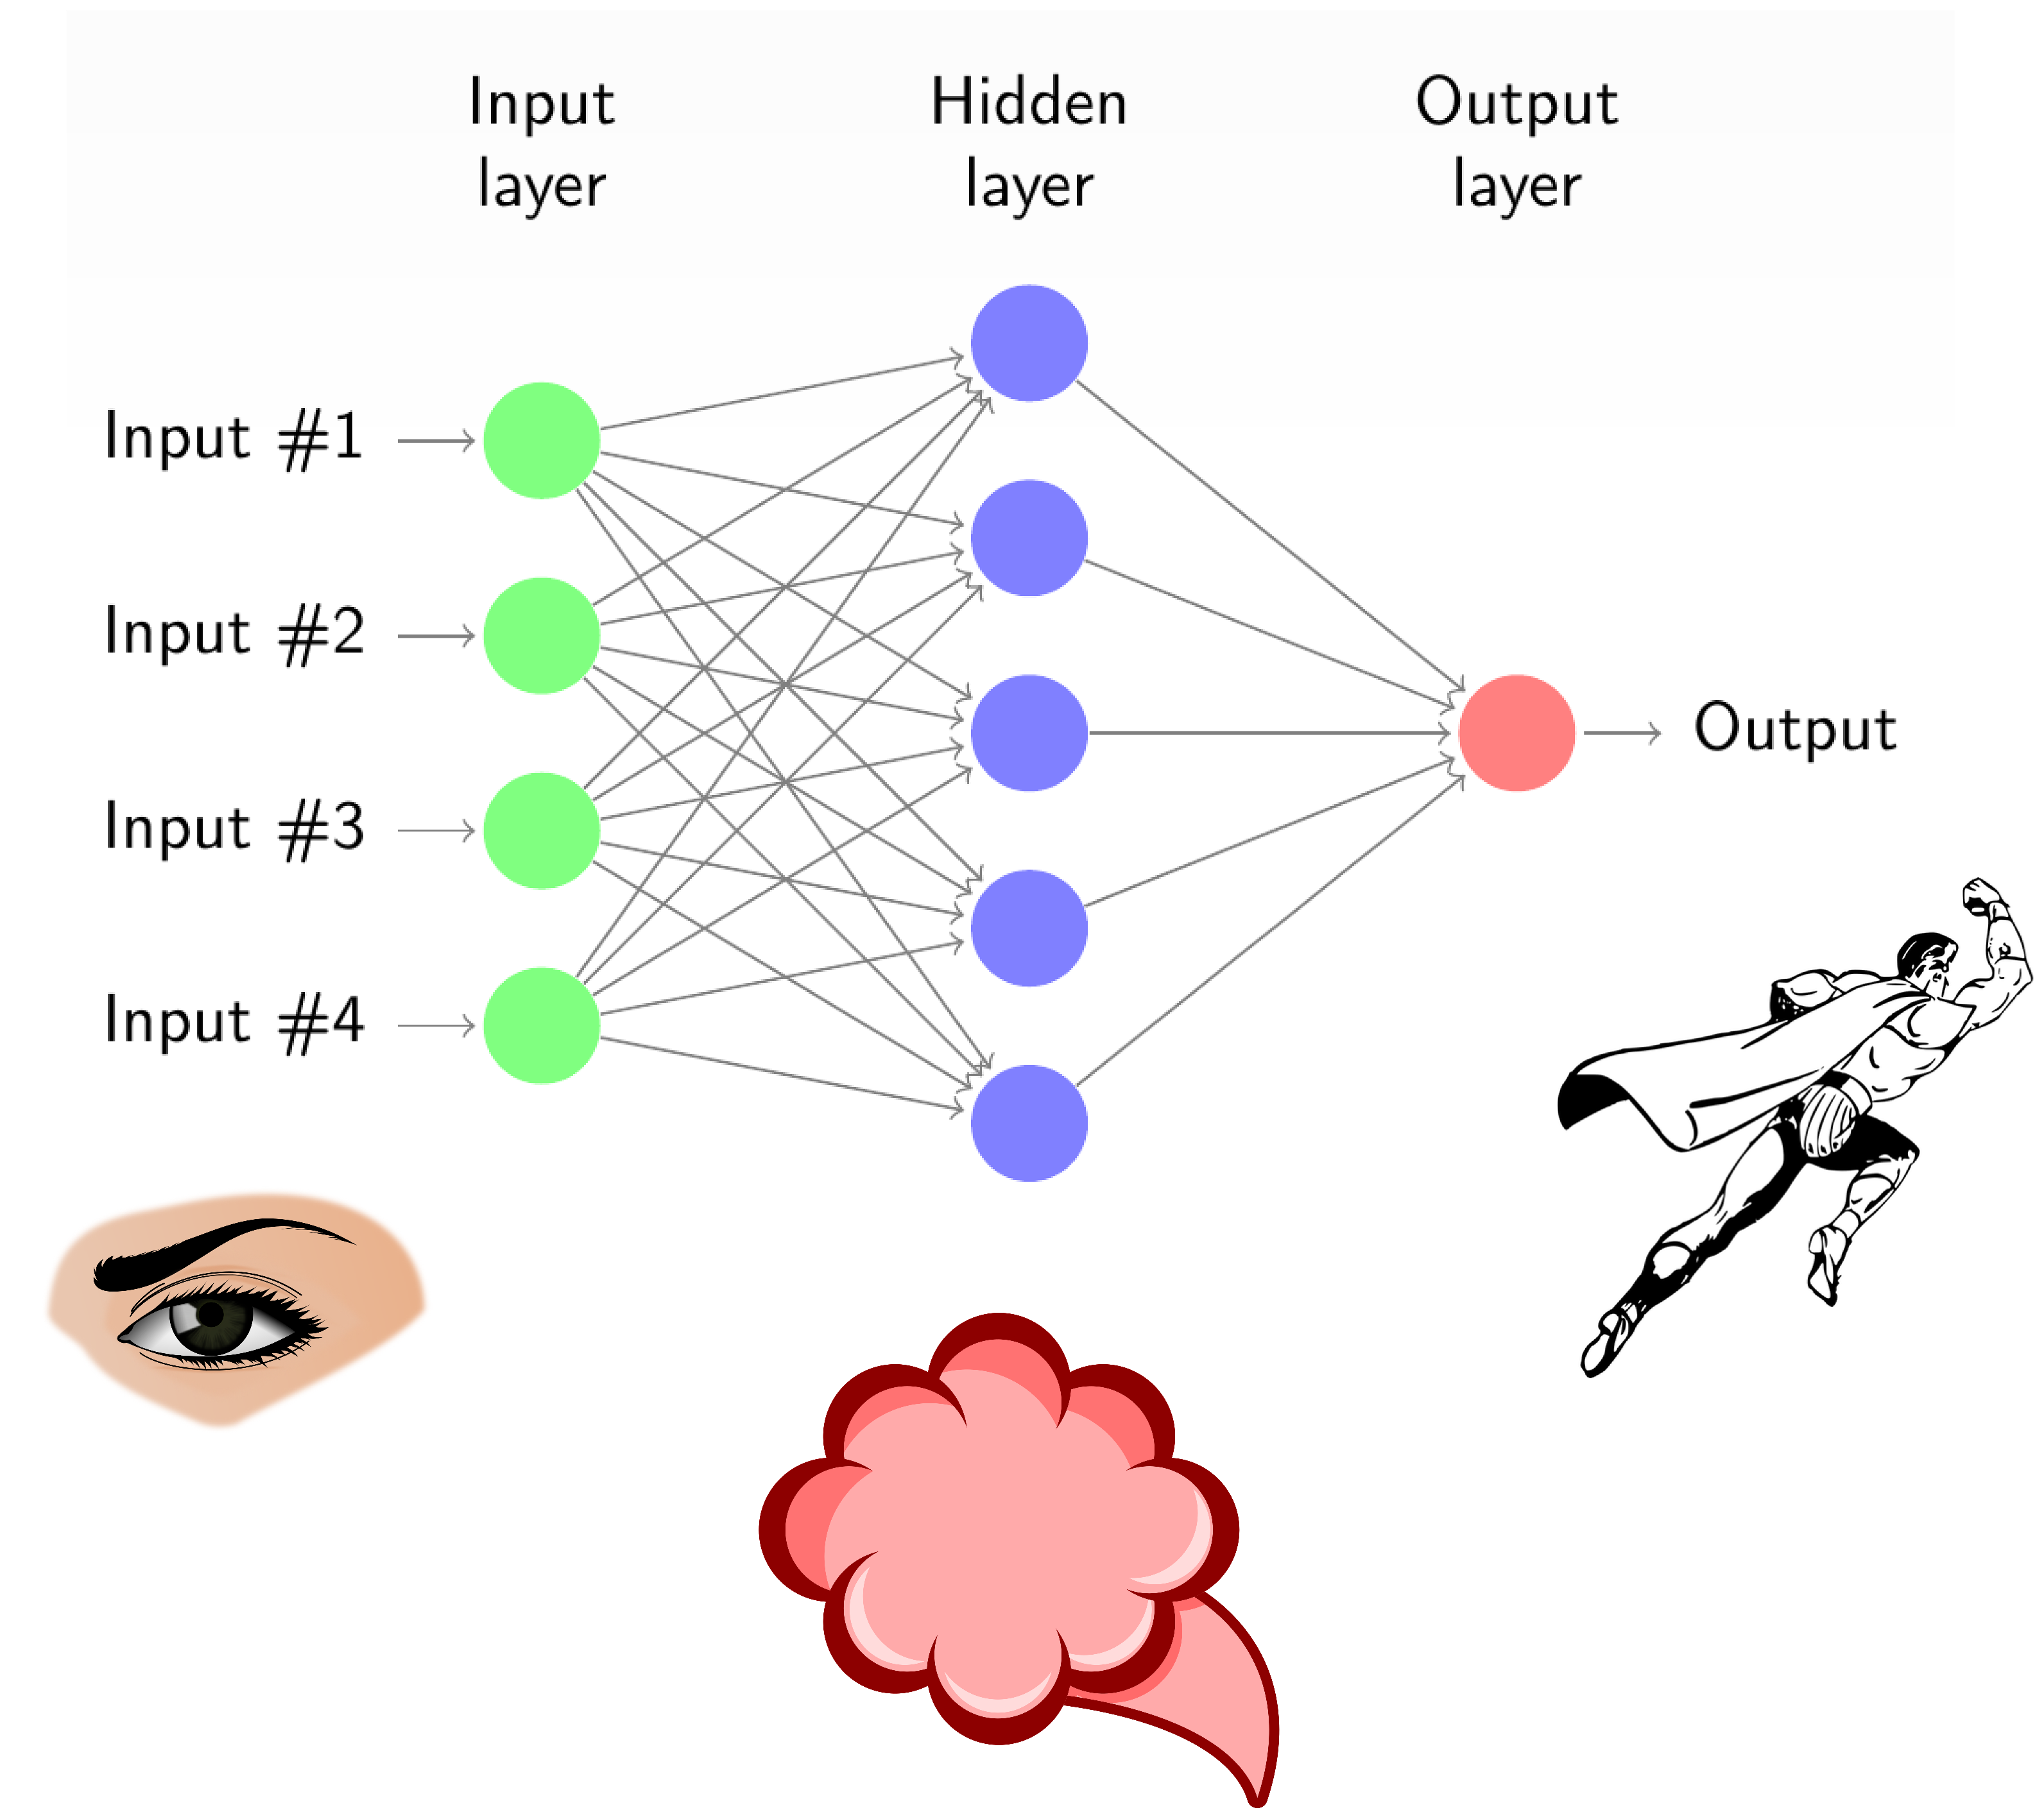
\includegraphics[width=0.8\textwidth]{net_structure}
\end{figure}
\end{frame}

\begin{frame}{Neural Networks - Choosing the next step}
\begin{tabular}{p{5cm}|p{5cm}}
    \begin{figure}
    	
\includegraphics[scale = 0.09]{brain}
    \end{figure}
    & 
    \begin{figure}
    	
\includegraphics[scale = 1.4]{machine}
    \end{figure} \\
  \multicolumn{1}{c|}{Evaluation of an action} & \multicolumn{1}{c}{Loss function} \\
    \begin{itemize}
        \item Simple perceptions: pain, satisfaction
        \item Expectation
    \end{itemize}
    & 
    \begin{itemize}
      \item Supervised learning: compare to the desired outcome
      \item Loss = estimator for quality
    \end{itemize} \\
\multicolumn{1}{c|}{Decision for a next step} & \multicolumn{1}{c}{Optimisation} \\
    \begin{itemize}
        \item Trial and error
        \item Learning from experience
    \end{itemize}
    & 
    \begin{itemize}
      \item Back-propagation impact of parameters' on the loss
      \item Adjust parameters to minimise plot
    \end{itemize} 
 \end{tabular}
\end{frame}

\begin{frame}{Hyperparameter optimisation}
    \begin{block}{What is a hyperparameter?}
        \begin{itemize}
            \item During the learning process the neural network optimises its internal parameters
            \item Some parameters are still set by the user according to the task of the network
            \item These are called hyperparameters
        \end{itemize}
        
    \end{block}
    \begin{block}{How does one optimise the choice?}
        \begin{itemize}
            \item Neural networks provide several metrics to estimate result and performance
            \item To optimise the hyperparameters one usually runs several configurations to find a good set of parameters
        \end{itemize}
    \end{block}
\end{frame}


\begin{frame}{Concepts of evolutionary network optimisation}
    \begin{block}{Choosing a start}
        \begin{itemize}
            \item Randomly choose a set of values for each hyperparameter
            \item Combine the random selection to create a set of network configurations
        \end{itemize}
    \end{block}
    \begin{block}{Evaluating a start}
        \begin{itemize}
            \item Run the networks for a small number of epochs
            \item Use networks' metrics to evaluate the performance
        \end{itemize}
    \end{block}
    \begin{block}{Choosing a next step}
        \begin{itemize}
            \item Rank networks by their metrics
            \item Reuse, mate and mutate networks
        \end{itemize}
    \end{block}
\end{frame}

\begin{frame}{The initial generation}
    \begin{block}{Current setup}
        \begin{itemize}
            \item Choose a random set of hyperparameters from a range of paramters set by the user
            \item Create a set of neural networks from all possible combinations
        \end{itemize}
    \end{block}
    \begin{block}{Planned}
        \begin{itemize}
            \item Draw each hyperparameter from a fitting distribution
            \item Restrict the number of combinations based on the hyperparameter
        \end{itemize}
    \end{block}
\end{frame}

\begin{frame}{Evaluating a generation}
    \begin{block}{Current setup}
        \begin{itemize}
            \item Evaluate all networks based on a metric of choice
            \item The metric of choice can be simply the AUC
            \item Save the $x$ best configuration
        \end{itemize}
    \end{block}
    \begin{block}{Planned}
        \begin{itemize}
            \item Test and combine different metrics
            \item Implement different metrics with regard to early stopping
        \end{itemize}
    \end{block}
\end{frame}

\begin{frame}{Breeding the next generation}
    \begin{block}{Current setup}
        \begin{itemize}
            \item Always keep the best configuration
            \item Recombine the $\lambda$ best configurations
            \item Recombine the $\lambda$ best generations again and vary $\mu$ hyperparameters
        \end{itemize}
    \end{block}
    \begin{block}{Planned}
        \begin{itemize}
            \item Include more hyperparameters
            \item Specify different variation probabilities and values for different hyperparameters
        \end{itemize}
    \end{block}
\end{frame}

\begin{frame}{Summary of the optimisation process}
    \begin{columns}
    \begin{column}{0.5\textwidth}
        \begin{itemize}
            \item Survival of the fittest: Keep the best setup
            \item Recombination: Reuse the best hyperparameters for the next batch
            \item Variation: Randomly change the hyperparamters to avoid local minima and bias
        \end{itemize}
    \end{column}
    \begin{column}{0.5\textwidth}
        \begin{figure}
            \centering
            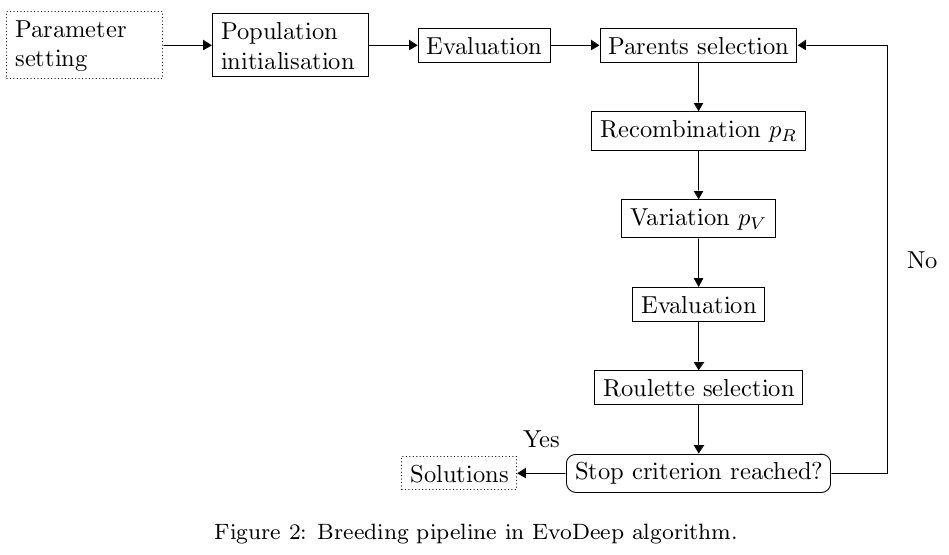
\includegraphics[width=\textwidth]{breed.png}
            \caption{\cite{naranjo}}
        \end{figure}
    \end{column}
    \end{columns}
\end{frame}
%\section{Results}
%Where are we?
%\begin{frame}{Conclusions}
    \begin{itemize}
        \item Neural networks in the \tHq channel is a \textbf{challenging} analysis.
        \vspace{0.2cm}
        \item \textbf{Negative} weights resulting from Monte Carlo generators \textbf{cannot} easily be handled by machine learning algorithms.
        \vspace{0.2cm}
        \item Different sizes of background samples result in smaller backgrounds getting \textbf{ignored} or even \textbf{misclassified} as signal.
        \vspace{0.2cm}
        \item Evolutionary optimisation of neural networks is a nice approach to \textbf{reoptimise} a network \textbf{automatically}.
    \end{itemize}
\end{frame}
\begin{frame}[plain,c]
%\frametitle{A first slide}

\begin{center}
\Huge Backup
\end{center}

\end{frame}

\begin{frame}{Evolutionary neural networks}
    \begin{itemize}
        \item Starting with a set of random configurations
        \vspace{0.2cm}
        \item Evaluate the results of the first generation and generate a new generation based on AUC 
        \vspace{0.2cm}
        \item Repeat until a good configuration is reached
        \vspace{0.2cm}
        \item Advantages:
            \begin{itemize}
                \item Decrease user bias for hyperparameter choice
                \item Optimised to run on worker nodes
                \item Quick discarding of bad configurations
                \item User friendly for unexperienced students
            \end{itemize}
    \end{itemize}
\end{frame}

%\begin{frame}{Inner product}
%    \begin{equation*}
%        a^{\mu} = \begin{pmatrix}
%            p_T \cosh ( \eta ) \\
%            p_T \cos ( \phi ) \\
%            p_T \sin ( \phi ) \\
%            p_T \sinh ( \eta ) \end{pmatrix}
%    \end{equation*}
%    %
%    \begin{align*}
%        \langle A | B \rangle = A_{\mu} B^{\mu}\\
%        = p_{T,A} p_{T,B} ( \cosh ( \eta_A ) \cosh ( \eta_B ) - \cos ( \phi_A ) \cos ( \phi_B)\\
%        - \sin ( \phi_A ) \sin ( \phi_B ) -\sinh ( \eta_A ) \sinh ( \eta_B ) )\\
%        = p_{T,A} p_{T,B} \left( \cosh ( \eta_A - \eta_B ) - \cos ( \phi_A - \phi_B ) \right)
%    \end{align*}
%\end{frame}

\begin{frame}{Responses}
  \begin{columns}
    \begin{column}{0.5\textwidth}
      \begin{figure}
      \centering 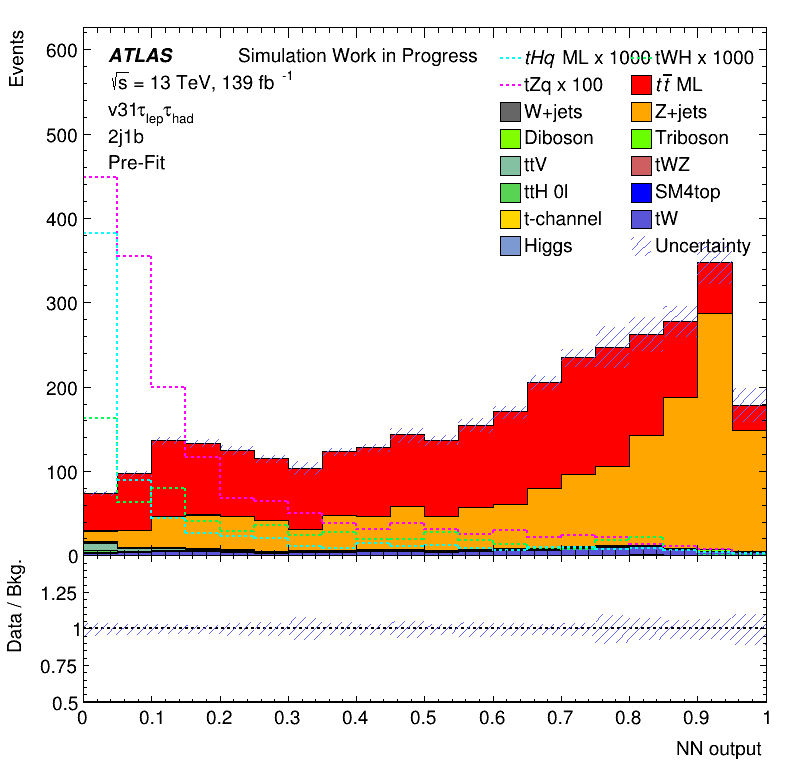
\includegraphics[width=\textwidth]{response_bkg}
      \caption{Background response}
      \end{figure}
    \end{column}
    \begin{column}{0.5\textwidth}
      \begin{figure}
      \centering 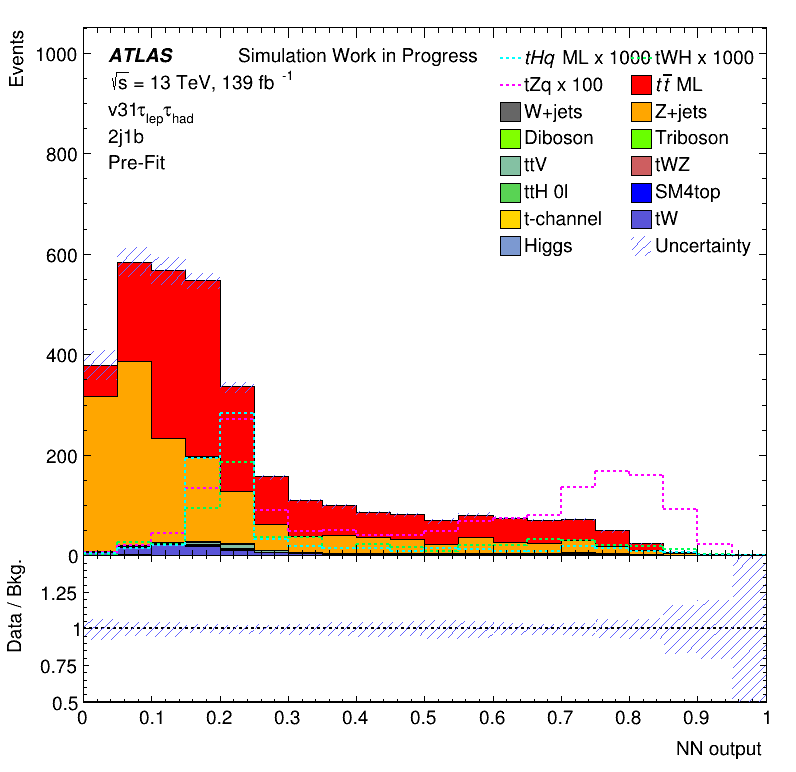
\includegraphics[width=\textwidth]{response_tZq}
      \caption{\tZq response}
      \end{figure}
    \end{column}
  \end{columns}
\end{frame}

\begin{frame}{\tHq versus \tZq}
  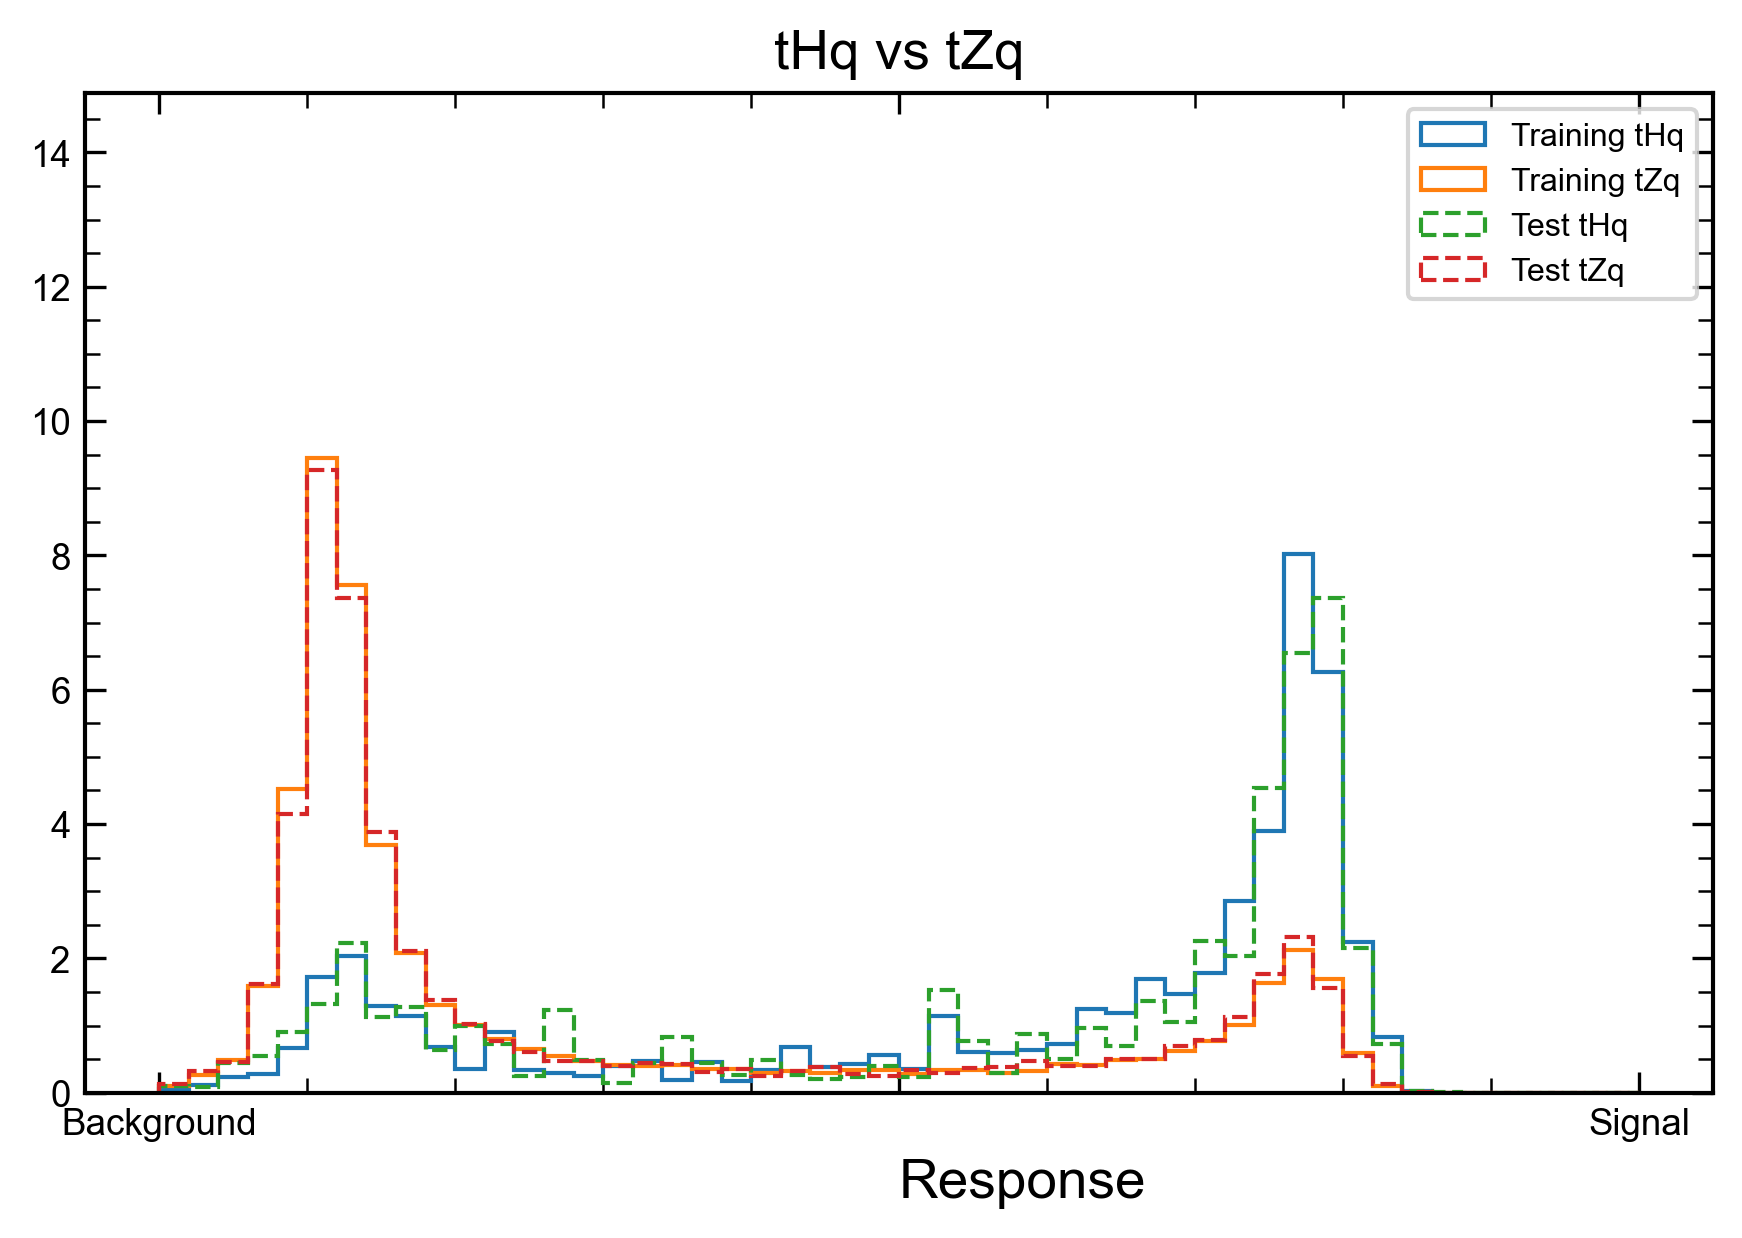
\includegraphics[width=\textwidth]{tHqvstZq.png}
\end{frame}

\begin{frame}{BDT summary}
    \begin{itemize}
        \item {\large A cut a bit below 0.2 would remove around 99\% of bkg
            events and 80\% of signal. Having just the 1\% of the bkg
            and 20\% of the signal would greatly increase our
            significance.}
        \vspace{0.2cm}
        \item {\large With the cut on the BDT we would have (approx.): bkg/sg = 4877/20 = 243
              Improved by a factor 71 to the before-presel scenario. Including BDT score in the trees}
        \vspace{0.2cm}
        \item {\large Using all events, not just the ones with positive weights reduces AUC surprisingly significantly}
        \vspace{0.2cm}
        \item {\large In the future the BDT should be tested in specific regions or for specific backgrounds}
    \end{itemize}
\end{frame}

\begin{frame}{}
  \centering 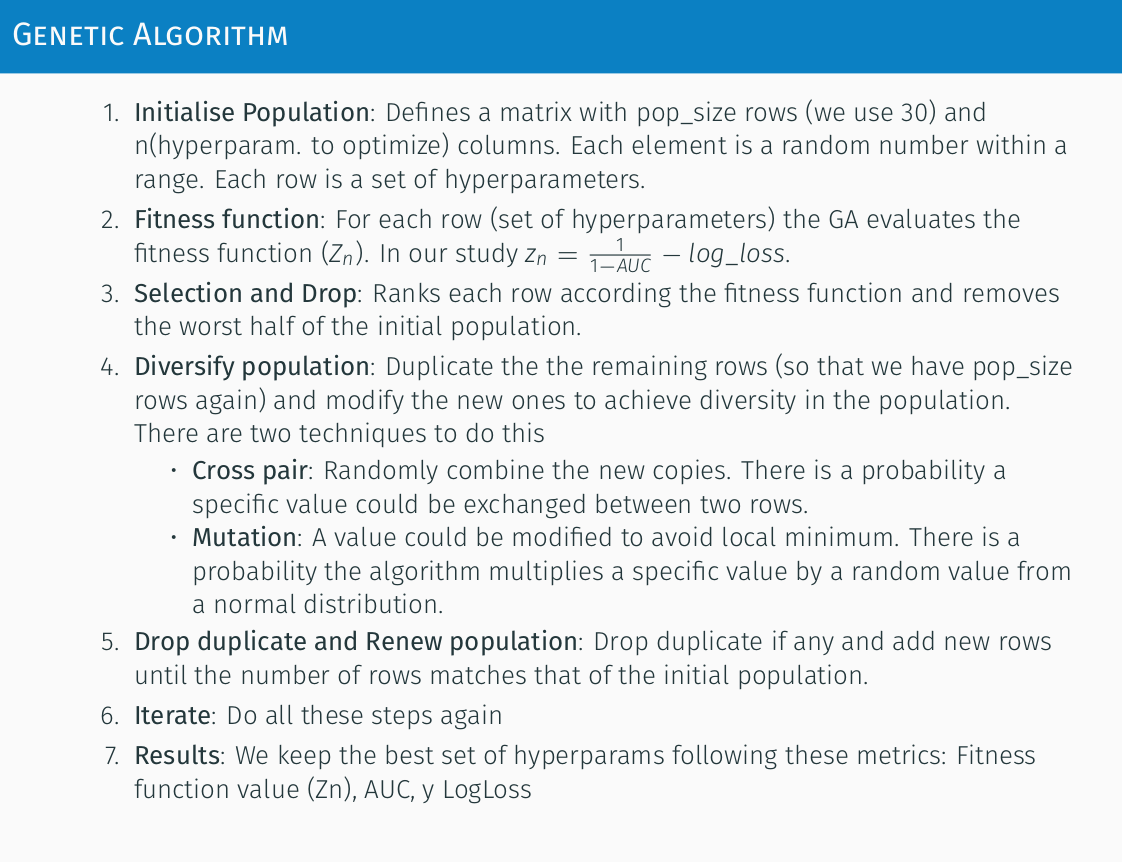
\includegraphics[width=\textwidth]{geneticAlg}
\end{frame}



\begin{frame}{Sources}

\printbibliography
    
\end{frame}






\end{document}